\documentclass[12pt,a4paper]{report}
\usepackage{cite}
\usepackage{longtable}
\usepackage[dvips]{graphicx,color}
\usepackage{makeidx}
\usepackage{nomencl}
\usepackage{float}
\usepackage{amsmath}
\usepackage{graphicx}
\usepackage{amssymb}
\usepackage{multicol}
\usepackage{dsfont}
\usepackage[bottom]{footmisc}\usepackage{subfigure}
\usepackage[OT2,OT1]{fontenc}
\linespread{1.3}
\newcommand{\imsize}{3in}
\renewcommand{\bibname}{References}
\newcommand{\norm}[1]{\left|\left|#1\right|\right|}
\newtheorem{definition}{Definition}
\newtheorem {remark}{Remark}
\newtheorem{thm}{Theorem}
\setlength{\textwidth}{6.3in}
\setlength{\textheight}{8.8in}
\addtolength{\oddsidemargin}{-0.5in}
\addtolength{\topmargin}{-0.2in}
\usepackage{tikz}
\usetikzlibrary{shapes,arrows,chains,matrix,positioning,scopes,decorations.pathmorphing,shadows,calc}


\begin{document}
	\begin{titlepage}
		\begin{center}
			{\bf\LARGE{NINE LEVEL INVERTER BASED ON SWITCHED CAPACITOR STRUCTURE}}\vspace{0.4in}\\
			{\Large{PROJECT REPORT}}\vspace{0.1in}\\
			{\large{Submitted by}}\vspace{0.4in}\\	
			{\bf\large ABHILASH M M (TCR15EE002)} \\
			{\bf\large ALIN ANTO (TCR15EE016)} \\
			{\bf\large DEVIKA SAJEEV (TCR15EE042)} \\
			{\bf\large DON DEV (TCR15EE046)}\vspace{0.2in}\\
			to\vspace{0.2in}\\
			The APJ Abdul Kalam Technological University\\
			in partial fulfillment of the requirements for the award of the degree\vspace{0.2in}\\
			of\vspace{0.2in}\\
			{\textit{Bachelor of Technology}}\\
			in\\
			{\textit{Electrical and Electronics Engineering}}\vspace{0.2in}\\
			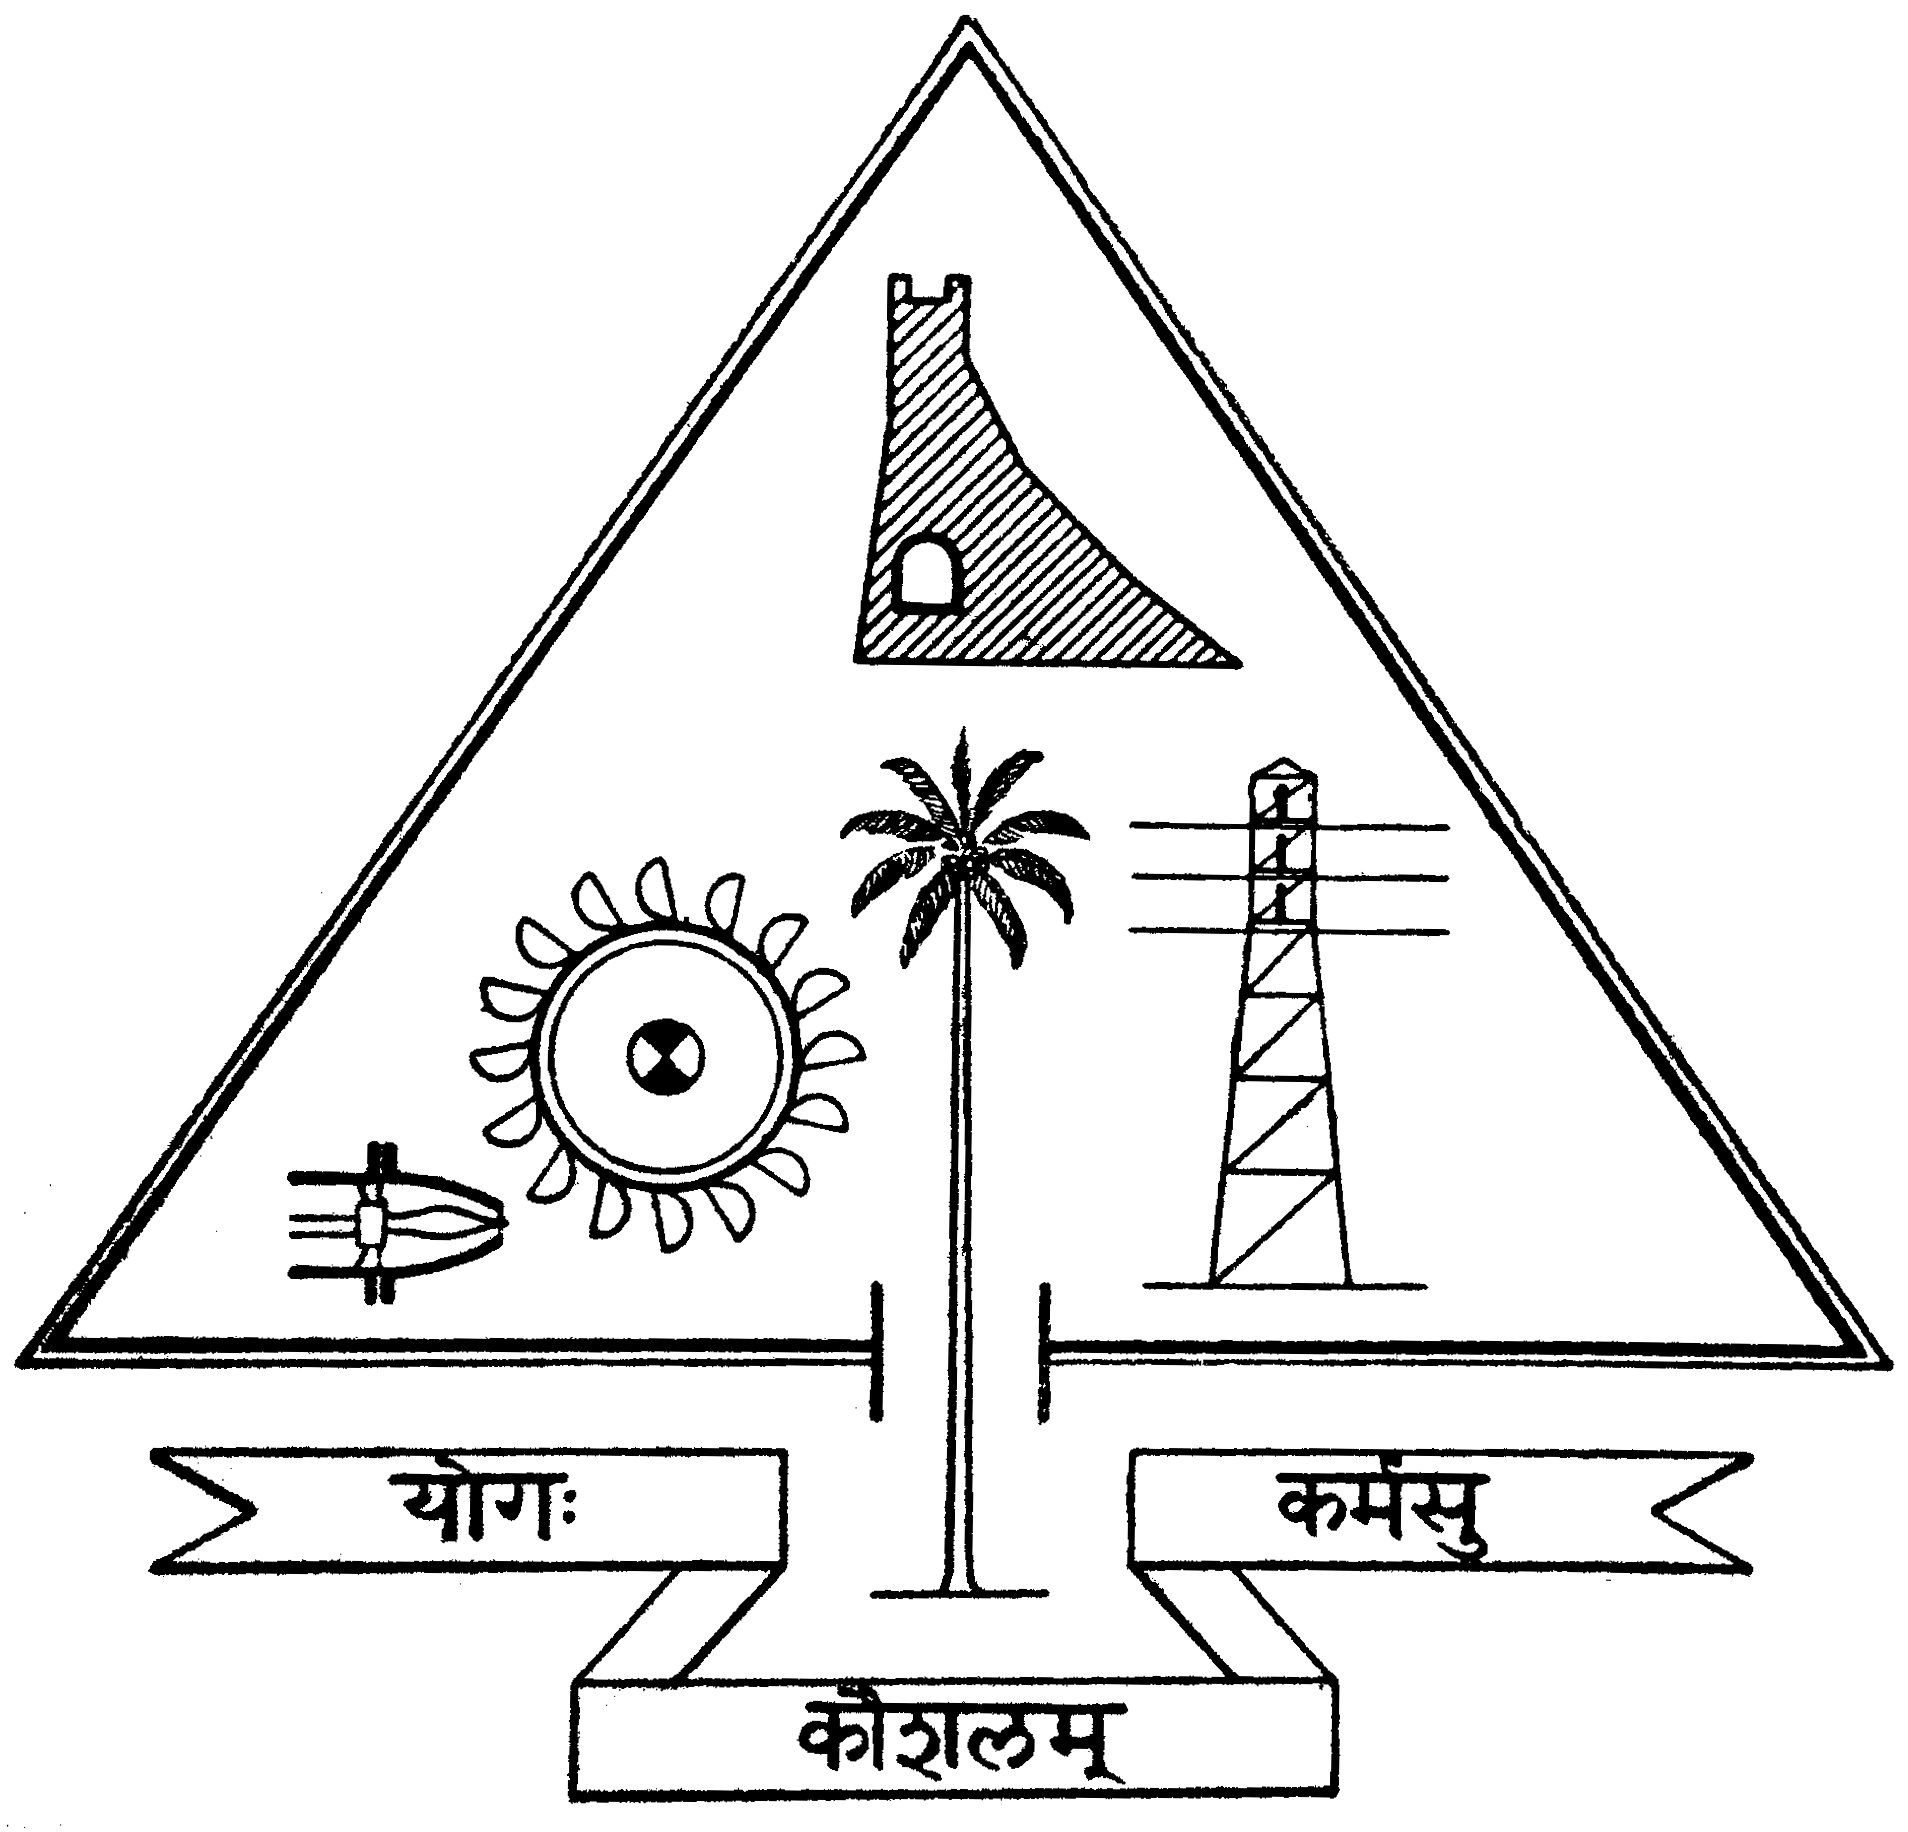
\includegraphics[height=1.8in, width=1.8in]{figures/gect.jpg}\\
			{\bf{Department of Electrical Engineering}} \\
			Government Engineering College, Thrissur  \\
			MAY - 2019\\
		\end{center}
	\end{titlepage}
	
\begin{center}
	\section*{DECLARATION}
\end{center}


	We undersigned hereby declare that the project report ( “Nine Level Inverter based on Switched Capacitor Structure”), submitted for partial fulfillment of the requirements for the award of degree of Bachelor of Technology of the APJ Abdul Kalam Technological University, Kerala is a bonafide work done by us under supervision of T.G. SANISH KUMAR, Associate Professor, Government Engineering College, Thrissur. This submission represents our ideas in our own words and where ideas or words of others have been included; we have adequately and accurately cited and referenced the original sources. We also declare that we have adhered to ethics of academic honesty and integrity and have not misrepresented or fabricated any data or idea or fact or source in our submission. We understand that any violation of the above will be a cause for disciplinary action by the institute and/or the University and can also evoke penal action from the sources which have thus not been properly cited or from whom proper permission has not been obtained. This report has not been previously formed the basis for the award of any degree, diploma or similar title of any other University. \\
	
	\begin{tabular}{lp{1.5in}r}
		Thrissur          &&  \textbf{ABHILASH MM}\\
		15/05/2019 &&  \textbf{ALIN ANTO}\\
						  &&  \textbf{DEVIKA SAJEEV}\\
						  &&  \textbf{DON DEV}\\
	\end{tabular}
	\thispagestyle{empty} 
	\clearpage
	



	
	\begin{center}
		{\Large \bf Department of Electrical Engineering}\\
		{\large \bf Government Engineering College, Thrissur}\\[.3 cm]
		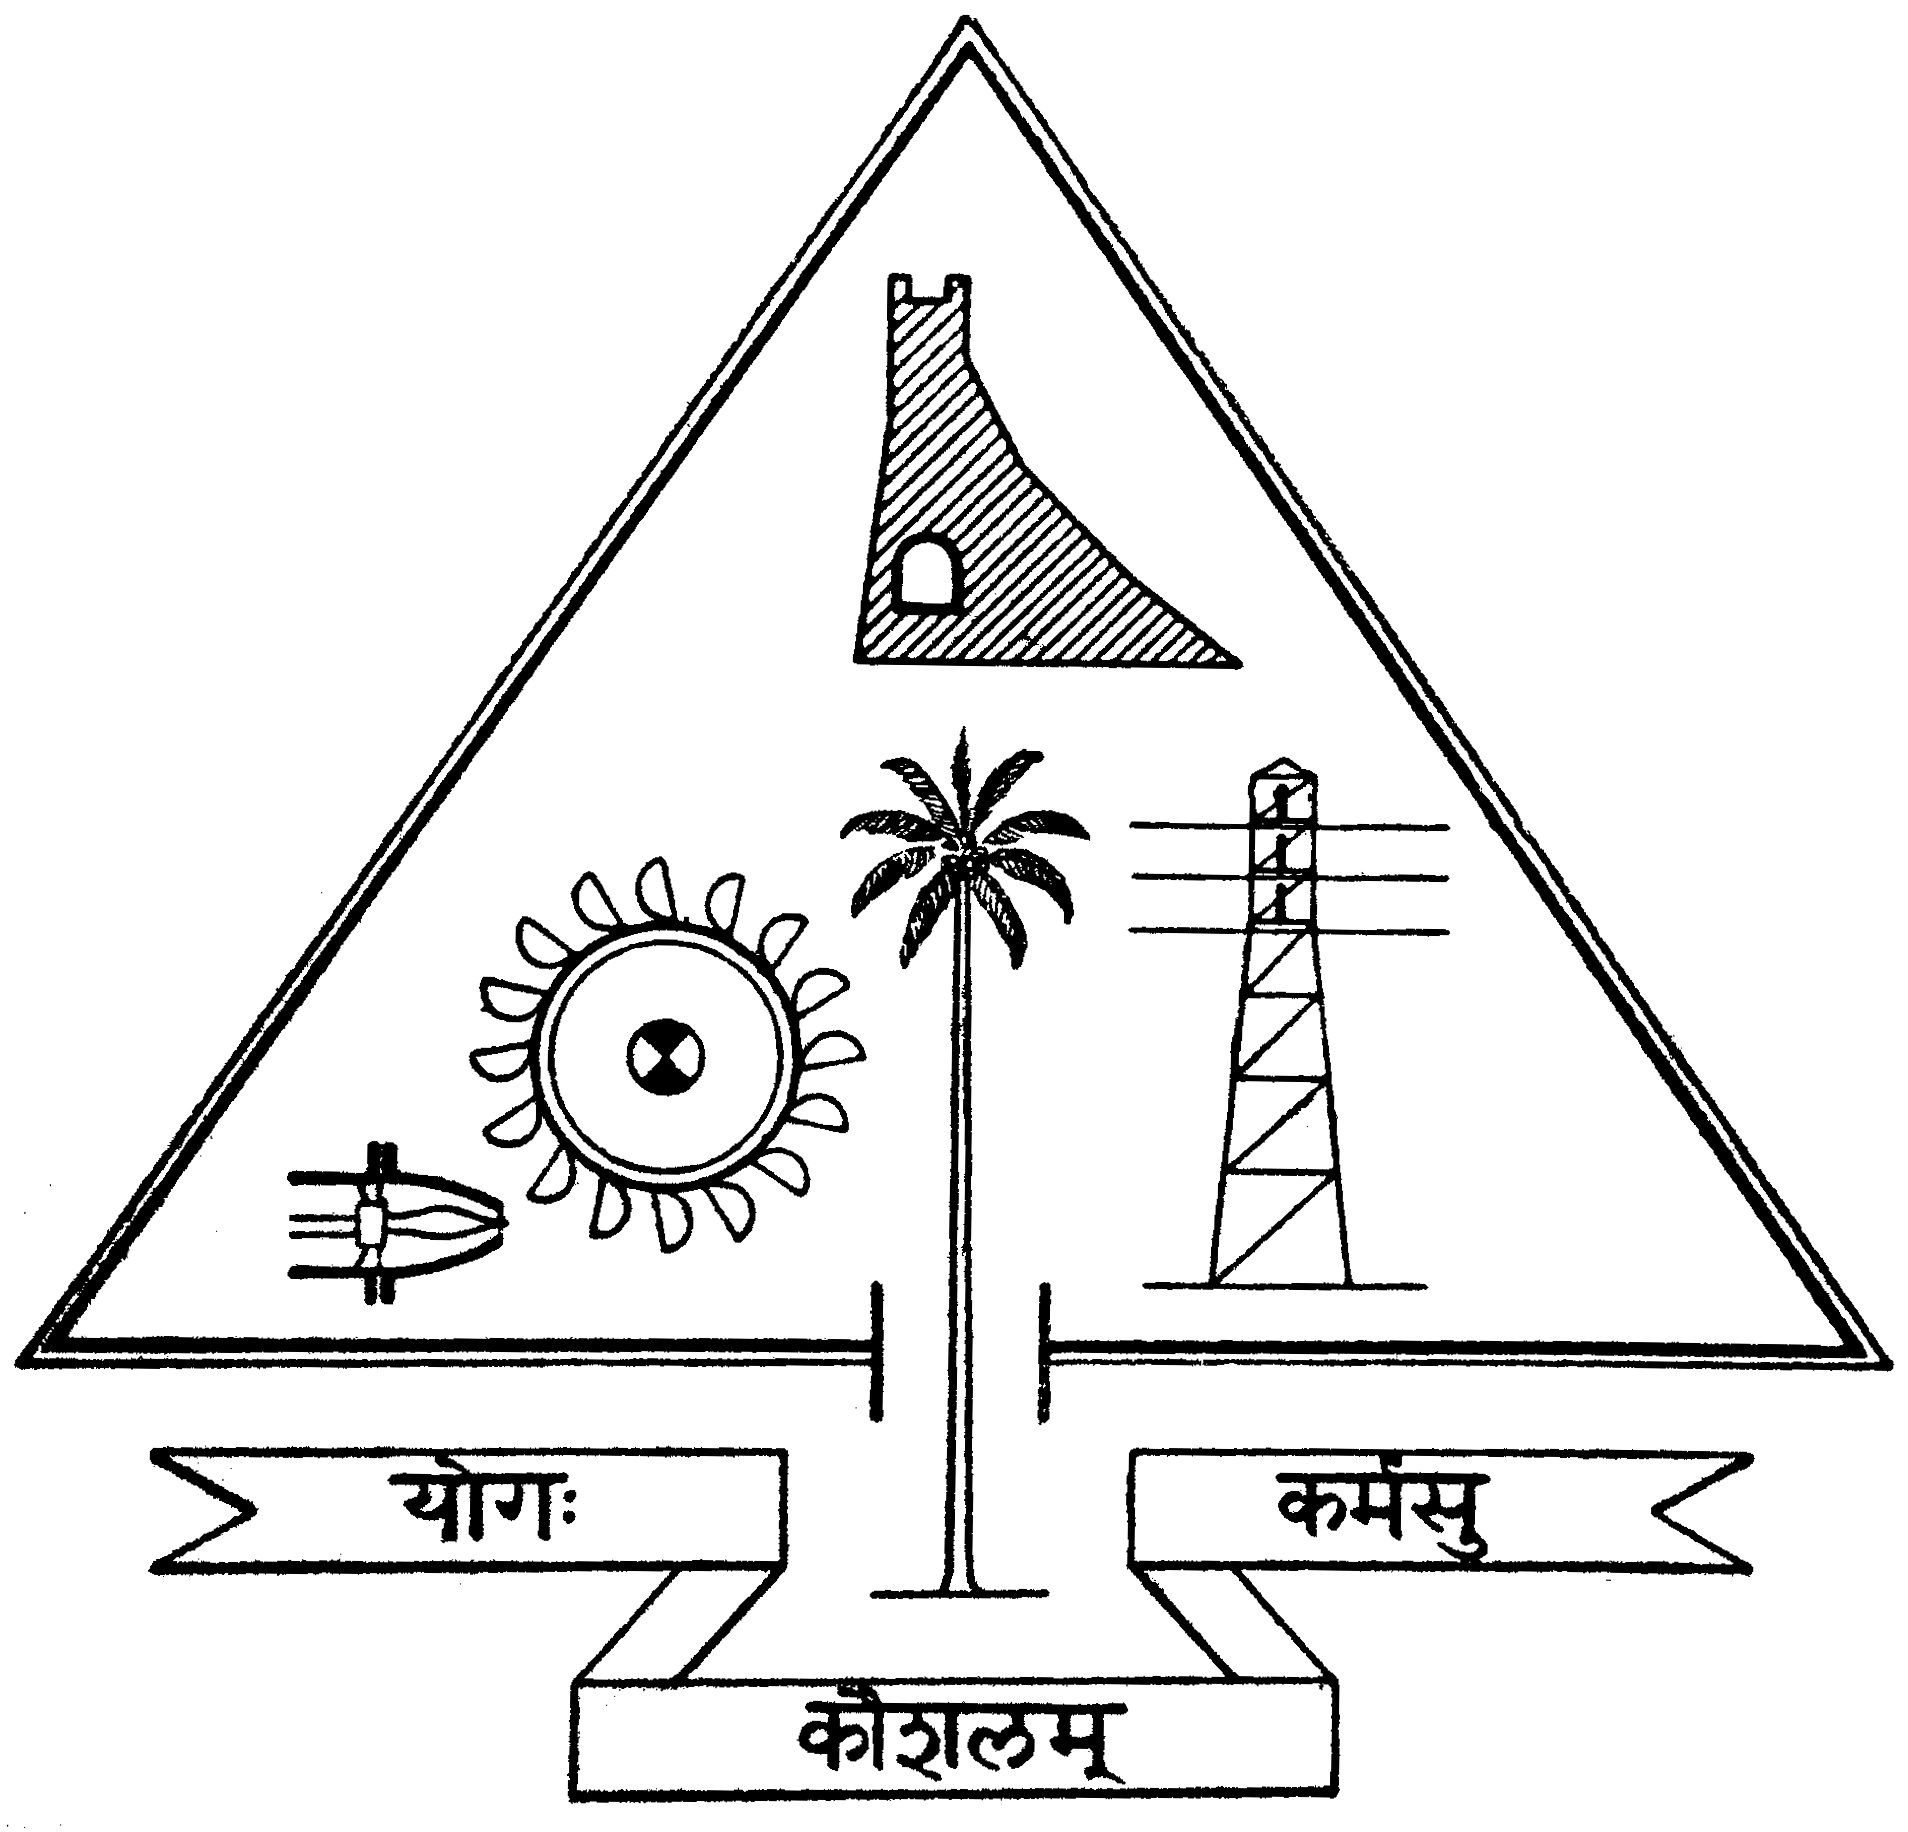
\includegraphics[width=4 cm]{figures/gect.jpg}\\[.3cm]
		\Large  \bf CERTIFICATE\\[0.1cm]
	\end{center}		
	\quad This is to certify that the Project Report titled {\bf ``NINE LEVEL INVERTER BASED ON SWITCHED CAPACITOR STRUCTURE"} is a bonafide record of the work carried out by {\bf ABHILASH M M (TCR15EE002), ALIN ANTO (TCR15EE016), DEVIKA SAJEEV (TCR15EE042), DON DEV (TCR15EE046)} to the APJ Abdul Kalam Technological University in partial fulfillment of the requirements for the award of the Degree of Bachelor of Technology (Electrical and Electronics Engineering) is a bonafide record of the project work carried out by them under my guidance and supervision. This report in any form has not been submitted to any other University or Institute for any purpose.\\ 

	\noindent{ Internal Supervisor } \\
	
	\noindent\begin{tabular}{lp{0.7in}r}
		T.G SANISH KUMAR         &&  Dr. REJI P\\
		Associate Professor &&  Head of Department\\
	    Dept. of Electrical Engineering	&&  Dept. of Electrical Engineering\\
		Govt. Engineering College, Thrissur &&  Govt. Engineering College, Thrissur\\
	\end{tabular}
	\thispagestyle{empty}
	\clearpage
	
\addcontentsline{toc}{chapter}{\quad ACKNOWLEDGEMENT}
\chapter*{ACKNOWLEDGEMENT\centering}
\par
\hspace{0.9cm}During the course of my project work several persons collaborated directly and indirectly with me. Without their support it would be impossible for me to finish my work. That is why I wish to dedicate this section to recognize their support.
\vspace {.2cm}
\par
\hspace{.35cm}I want to start expressing my thanks to my project guide {\bf T.G Sanish Kumar}, Associate Professor Dept. of Electrical Engineering, because of his valuable advice and guidance towards this work. I received motivation; encouragement and hold up from his during the course of work.
\vspace{.2cm}
\par 
\hspace{.35cm}I am thankful to {\bf Dr. Reji P}, 
Head of the Department, and our Principal {\bf Dr Sheeba V.S}, for their sole co-operation.
\vspace{0.2cm}
\par
\hspace{0.35cm}I am grateful to express my thanks to all the faculty members of our department for their support. I articulate my gratitude to all my associates and colleagues for their support and help for this work.
\vspace{0.2cm}
\par
\hspace{0.35cm}Last, but not the least I wish to express my gratitude to God Almighty for His abundant blessings without which this effort would not have been successful.\\
\thispagestyle{empty}
\clearpage

\addcontentsline{toc}{chapter}{\quad ABSTRACT}
\chapter*{ABSTRACT\centering}
Multilevel inverter is a power electronic device capable of providing desired output using multiple lower level DC voltages as an input. Multilevel inverters are gaining popularity over conventional two level inverters because it can produce a smoother stepped output waveform. Moreover, the output obtained from multilevel inverters has lower $dv/dt$ and lower harmonic distortions. Multilevel inverters usually make use of diode clamped, flying capacitor or cascaded H-bridge topologies. These topologies suffer from disadvantages such as multitude of components, large size and cost as well as complex control. This project aims to use a switched-capacitance (SC) structure to overcome the disadvantages of the existing topologies. It involves adding an SC structure to the H-bridge inverter using capacitors, switches and diodes to create a multilevel DC voltage at the DC bus of the H-bridge circuit. The proposed technology will improve upon the existing technology by having boost operation without magnetic elements, fewer components, less complex control and using only one power DC source. This project work involves the simulation and hardware implementation of Nine level Inverter based on Switched Capacitance Structure.
\thispagestyle{empty}
\clearpage

\tableofcontents
\clearpage
\addcontentsline{toc}{chapter}{\quad LIST OF FIGURES}
\listoffigures
\clearpage
\addcontentsline{toc}{chapter}{\quad LIST OF TABLES}
\listoftables
\clearpage

\chapter{INTRODUCTION}

\section{GENERAL BACKGROUND}
\hspace{0.2cm} Recently, multilevel inverters (MIs) are getting more attention from researchers because of advantages like better waveform quality, lower EM noise, and lower device stress. MIs are used to couple a DC source to an AC bus for applications like electric motor drivers, uninterruptible power supplies, and distributed generation systems. The following topologies are now used in practice:-\\

\noindent1$)$Neutral-point clamped (Diode clamped).\\
2$)$Flying capacitor.\\
3$)$Cascaded H-bridge (CHB).\\

\section{OBJECTIVE}

\noindent For low-power applications, the system size and cost are the main concerns.
Problems in multilevel inverters (MIs) employing current topologies are the following:-\\

\noindent1$)$Large number of components( switches, power supplies, capacitors, and diodes).\\
2$)$Large size and high cost.\\
3$)$Complex control.\\

\noindent Solution to the problem is a new MI topology that uses a Switched Capacitor(SC) structure in cascade with an H-bridge. The objective of this new system is to achieve the following characteristics for a  SC-MI:-\\

\noindent1$)$Fewer components(switches, sources and capacitors).\\
2$)$Smaller and less expensive.\\
3$)$Less complex control.\\
4$)$Requires only one power DC source.\\
5$)$Boost operation without magnetic elements.\\
	
\section{SCOPE}	

Future holds immense scope for multi-level inverters. The electronic devices in the future which may comprise entirely of ICs and other microprocessors would require very high standards of power quality which may not be realistically conceived by means of the existing inverter topologies. Also, the existing MI topologies are bulky, complex to control and expensive. The switched capacitance topology is however, easy to control and cheap while using lesser number of switches.
With further research and development, mutli-level inverters may take over the market for inverters in the growing electronic industry.

\section{REQUIREMENTS}

\begin{table}[h!]
	\centering
	\begin{tabular}{|c|c|} 
		\hline
		{\bf Hardware Requirements} & {\bf Software Requirements} \\  
		\hline
		DSO (Analysis) & Matlab (Simulation) \\ 
		\hline
		DSP (controller) & Proteus (Design) \\
		\hline
		Function generator (Analysis and reference) & Latex (Documentation) \\
		\hline
		
		
	\end{tabular}
	\caption{System Requirements}
	

\end{table}

\chapter{LITERATURE SURVEY}

 
The Multilevel inverter is a novel concept emerging as a promising advancement in the field of inverters since they provide features like fewer components, smaller and less expensive system, less complex control, etc. 
The existing researches have implemented multilevel inverters using techniques like cascaded H-bridge, diode clamped, flying capacitor structure, etc. Multilevel inverters have an arrangement of power switching
devices and capacitor voltage sources. Multilevel inverters are suitable for
high-voltage applications because of their ability to synthesize output voltage
waveforms with a better harmonic spectrum and attain higher voltages with a
limited maximum device rating.\\

 
Balancing among dc link and clamping capacitors exists in
both neutral point clamped and flying capacitor inverters.
Diode clamped or neutral clamped has the difficulty of increase
in the number of clamping diodes as the level increases.
Similarly, in flying capacitor the number of capacitors
increases and system becomes bulkier. Among these inverter
topologies cascaded inverter achieves greater reliability and
simplicity.\\


A multilevel inverter has several advantages over a conventional
two-level inverter that uses high switching frequency pulse width modulation
(PWM). The most attractive features of a multilevel inverter are as follows:\\
1) They can generate output voltages with extremely low
distortion and lower dv/dt.\\
2) They draw input current with very low distortion.\\
3) They generate smaller common-mode (CM) voltage.\\
4) They can operate with a lower switching frequency.\\

\par 
Multilevel inverters have an arrangement of power switching
devices and capacitor voltage sources. Multilevel inverters are suitable for
high-voltage applications because of their ability to synthesize output voltage
waveforms with a better harmonic spectrum and attain higher voltages with a
limited maximum device rating.
\par
There are three main types of multilevel inverters: diode-clamped
(neutral-clamped), capacitor-clamped (flying capacitors), and cascaded H-bridge
inverter.

\section{Diode Clamped Structure}

The diode-clamped inverter is also known as the neutral-point
clamped inverter (NPC) which was introduced by Nabae et al (1981). The
diode-clamped inverter consists of two pairs of series switches (upper and
lower) in parallel with two series capacitors where the anode of the upper
diode is connected to the midpoint (neutral) of the capacitors and its cathode
to the midpoint of the upper pair of switches; the cathode of the lower diode is
connected to the midpoint of the capacitors and divides the main DC voltage
into smaller voltage.\\

\begin{figure}[h]\centering
	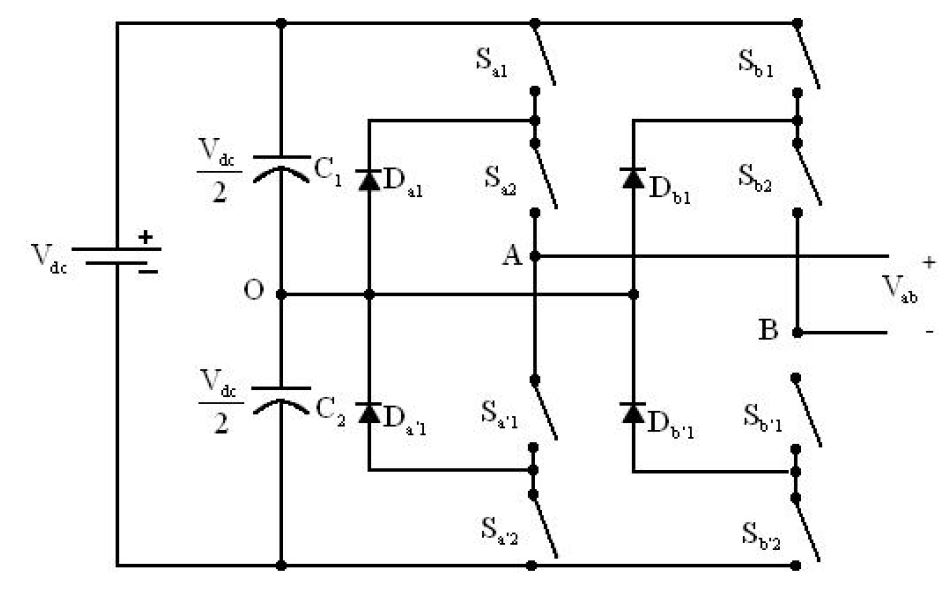
\includegraphics[width=12cm,height=7cm]{figures/diode.jpg}
	\caption{Two phase diode clamped multilevel inverter}
	\label{diode}
\end{figure}
 The middle point of the two capacitors can be defined as the “neutral point”. The NPC uses a single
dc bus that is subdivided into a number of voltage levels by a series string of
capacitors. For a three-level diode-clamped inverter if the point O is taken as
the ground reference, the output voltage has three states
0, +1/2$V_{dc}$ and -1/2$V_{dc}$.
The line-line voltages of two legs with the capacitors are: 0, +1/2$V_{dc}$, -1/2$V_{dc}$, +$V_{dc}$, -$V_{dc}$.Three phases are necessary to generate a three-phase voltage.\\

The disadvantages of this system are,\\
(1) Different voltage ratings for clamping diodes are required.\\
(2) Real power flow is difficult because of the capacitors
imbalance.\\
(3) Need high voltage rating diodes to block the reverse voltages.\\
(4) The number of switches, capacitors, and diodes required in
the circuit increases with the increase in the number of output
voltage levels. Extra clamping diodes required are
n 1 n 2 per phase.\\

\section{Capacitor-Clamped Inverter}
Capacitor-clamped multilevel inverter topologies are relatively new
compared to the diode-clamped or the cascaded H-bridge cell inverter
topologies. Redundancy in the switching states is available by using flying
capacitors instead of clamping diodes. This redundancy can be used to
regulate the capacitor voltages and obtain the same desired level of voltage at
the output. Figure 2.2 shows a single-phase five-level capacitor-clamped
multilevel inverter topology. The voltage across the capacitors is considered
to be half of DC source voltage $V_{dc}$. The output voltage consists of five
different voltage levels,  0, +1/2$V_{dc}$, -1/2$V_{dc}$, +$V_{dc}$, -$V_{dc}$.
Similar to the other multilevel inverter topologies, capacitor clamped
multilevel inverter also has complementary pairs of switches. The number of switching states for the
capacitor-clamped multilevel inverter topology is higher than that of the
diode-clamped inverter. The number of voltage levels at the output can be
increased by adding a pair of complementary switches and a capacitor. An
output voltage can be produced by using different combinations of switches.
The topology allows increased flexibility in how the majority of the voltage
levels may be chosen. In addition, the switches may be chosen to charge or
discharge the clamped capacitors, which balance the capacitor voltage.

\begin{figure}[h]
	\centering
	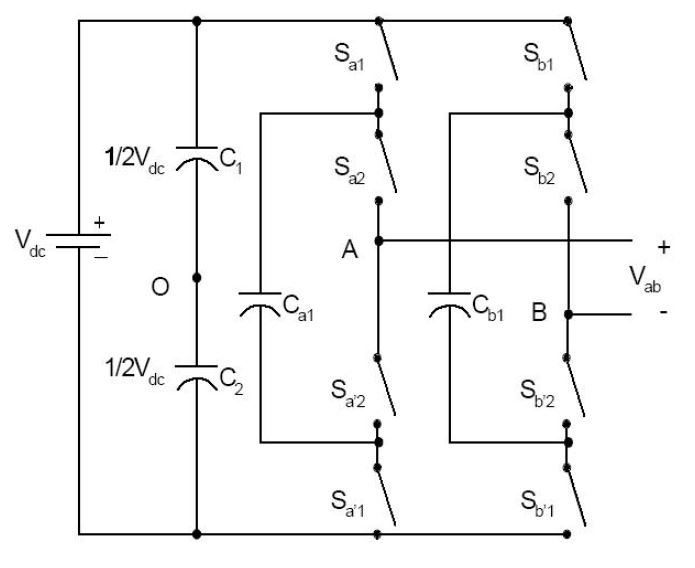
\includegraphics[width=12cm,height=7cm]{figures/capac.jpg}
	\caption{Capacitor-Clamped Multilevel Inverter}\label{capacitor}
\end{figure}
\vspace{1.0cm}
The disadvantages are,\\
(1) Large numbers of capacitors are bulky and more expensive
than the clamping diodes used in the diode-clamped
multilevel inverter.\\
(2) Complex control is required to maintain the capacitor’s
voltage balance.\\
(3) Switching utilization and efficiency are poor for real power
transmission.\\

\section{Cascaded H-Bridge Inverter}
The cascaded H-bridge inverter has drawn tremendous interest due
to the greater demand of medium-voltage high-power inverters. The cascaded
inverter uses series strings of single-phase full-bridge inverters to construct
multilevel phase legs with separate dc sources. The output of each H-bridge can have three discrete levels, results
in a staircase waveform that is nearly sinusoidal even without filtering. A
single H-bridge is a three-level inverter. Each single-phase full-bridge
inverter generates three voltages at the output: +$V_{dc}$,0 and -$V_{dc}$.
The four switches $S_{1}$, $S_2$ ,$S_3$ and $S_4$ are controlled to generate three
discrete outputs out V with levels  +$V_{dc}$,0 and -$V_{dc}$. . When $S_1$ and $S_2$ are on, the
output is $V_{dc}$ ; when $S_3$ and $S_4$ are on, the output is -$V_{dc}$.

\begin{figure}[h!]\centering
	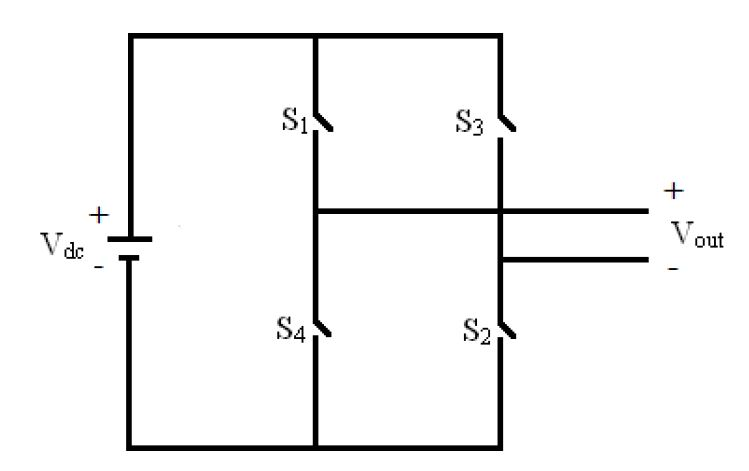
\includegraphics[width=12cm,height=7cm]{figures/hbridge.jpg}
	\caption{Single H-Bridge Topology}\label{hbridge}
\end{figure}

The disadvantage for cascaded multilevel H-bridge inverter is the
following:\\
(1) Needs separate DC sources.\\
(2) Needs large number of switches. \\

This project presents a multilevel inverter based on switched capcitance structure which can generate a greater number of voltage levels with optimum number of components.\\
\cleardoublepage

\chapter{SWITCHED CAPACITOR NINE LEVEL INVERTER}

This chapter discusses the working of a switched capacitor based nine level inverter with reduced switch count and a single DC source. It also explains the phase disposition PWM technique used to generate the switching signals for the inverter.

 \begin{figure}[h!]
 	\begin{center}
 		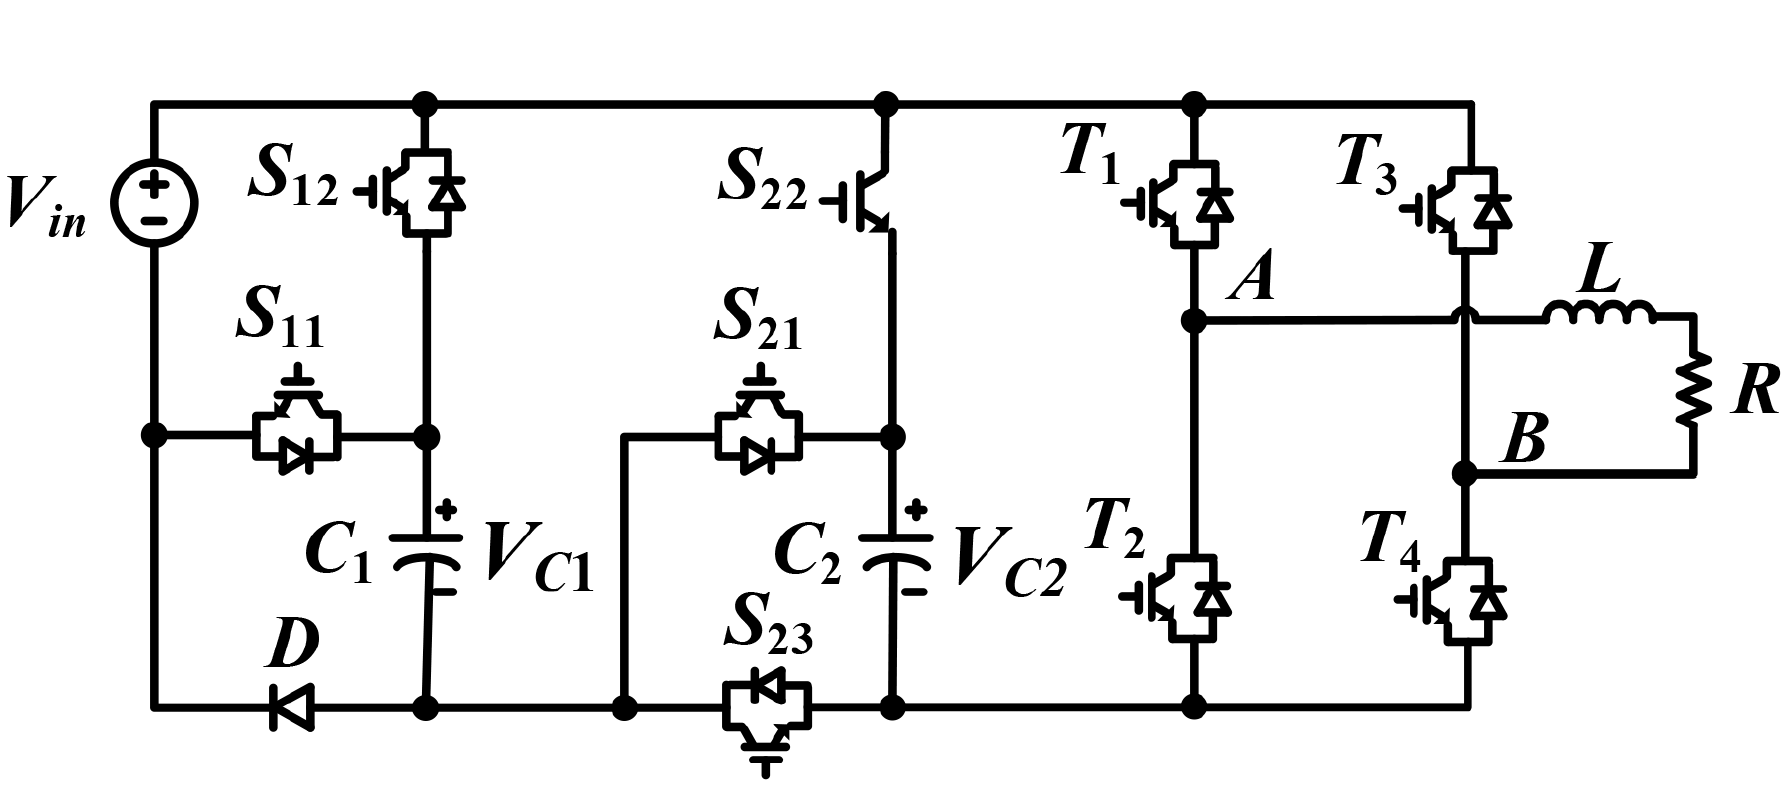
\includegraphics[width=16cm,height=7cm]{figures/Main_Circuit}
 	\end{center}
 	\caption{Switched Capacitor 9-level inverter circuit}
 	\label{sc}
 	
 \end{figure}
 
 \hspace{0.2cm} The proposed inverter consists of a single DC source, two SC cells connected in parallel with the H-bridge circuit and a load. The first SC cell is a combination of one capacitor, one diode, and two switches ($C_1-D-S_{11}-S_{12}$), and the second SC cell includes one capacitor, and three switches ($C_2-S_{21}-S_{22}-S_{23}$). Switched capacitor is the most famous voltage boosting technique. This technique uses capacitor in conjuction with power semiconductor switches. A voltage doubler is an electronic circuit which charges capacitors from the input voltage and switches these charges in such a way that, in the ideal case, exactly twice the voltage is produced at the output as at its input. The simplest of these circuits are a form of rectifier which take an AC voltage as input and outputs a doubled DC voltage. The switching elements are simple diodes and they are driven to switch state merely by the alternating voltage of the input. DC-to-DC voltage doublers cannot switch in this way and require a driving circuit to control the switching. They frequently also require a switching element that can be controlled directly, such as a transistor, rather than relying on the voltage across the switch as in the simple AC-to-DC case. Cascading identical stages together achieves a greater voltage multiplication. A comparison of the number of components used in realising a 9 level inverter using switched capacitor structure and other conventional topologies are summarised in the table below.\\
 
 \begin{table}[H]
	\begin{center}
		\begin{tabular}{|c|c|c|c|c|} 
			\hline
			{\bf Topology} & {\bf Capacitor} & {\bf Diode} & {\bf Switch} & {\bf DC Source} \\  
			\hline
			Switched Capacitor MLI & 2 & 2 & 9 & 1 \\ 
			\hline
			Diode clamped MLI & 8 & 28 & 32 & 1 \\
			\hline
			Flying Capacitor MLI & 64 & 0 & 32 & 1 \\
			\hline
			Cascaded H-Bridge MLI & 0 & 0 & 16 & 4 \\
			\hline
		\end{tabular}
	\end{center}
	\caption{Comparison of the number of components in a 9 level inverter}
\end{table}

\section{Switched Capacitor Structure}

Capacitor $C_1$ is charged while connected in parallel with the input source through $S_{12}$. It is discharged in series with the input source through $S_{11}$. Capacitor $C_2$ is charged in parallel from the input source and capacitor $C_1$ through $S_{22}$ and $S_{23}$. It is discharged in series with capacitor $C_1$ and the input source through $S_{21}$. $C_1$ is thus charged to $V_{in}$ and $C_2$ is charged to $2V_{in}$. Four Levels of voltage (in addition to a zero level) are therefore obtained by the following combinations:-\\

\begin{table}[h!]
\begin{center}
	\begin{tabular}{|c|c|c|} 
		\hline
		{\bf MODE} & {\bf OUTPUT VOLTAGE} & {\bf STATE} \\  
		\hline
		1 & $V_{in}$  & Source and $C_1$ in parallel. \\ 
		\hline
		2 & $2V_{in}$ & Source and $C_1$ in series, then parallel with $C_2$. \\
		\hline
		3 & $3V_{in}$ & Source and $C_1$ in parallel, then series with $C_2$. \\
		\hline
		4 & $4V_{in}$ & Source, $C_1$ and $C_2$ all in series. \\
		\hline
	\end{tabular}
\end{center}
\caption{Output voltage states}
\end{table}

In mode 1, the voltage across $C_1$ and that of voltage source $V_{in}$ are equal and parallel. In mode 2, the voltage source $V_{in}$ and the voltage across $C_1$ (which is $V_{in}$) are connected in series due to the configuration and switching ON of the curresponding switches. Thus, the second output voltage stage, i.e. 2$V_{in}$ is obtained. In mode 3, the voltage source $V_{in}$ and the capacitor $C_1$ are in parallel which makes the effective voltage across the parallel block to be $V_{in}$. The capacitor was charged to a voltage of 2$V_{in}$ in the previous cycle. Hence, a series connection between the parallel block and the capacitor $C_2$ produces the additive sum of the parallel block and the capacitor $C_2$ to produce a voltage 3$V_{in}$. In mode 4, the voltage source $V_{in}$ and the capacitor $C_1$ are in series which produces a voltage equal to 2$V_{in}$ in the series network. This network is connected in series with capacitor (charged to voltage 2$V_{in}$). The cumulative voltage across the series connected networks is 4$V_{in}$, which appears as the fourth voltage stage. \\

\section{Modes of Operation}

\begin{figure}[h!]
	
	\includegraphics[width=16.5cm,height=10cm]{figures/Mode}
	\caption{Modes of operation}
	\label{moo}
\end{figure}

In mode 1, the voltage across $C_1$ and that of voltage source $V_{in}$ are equal and parallel. Hence, the total voltage that is produced across the load is same as $V_{in}$. This is the first output voltage stage. \\

In mode 2, the voltage source $V_{in}$ and the voltage across $C_1$ (which is $V_{in}$) are connected in series due to the configuration and switching ON of the curresponding switches. This results in additive sum of the voltage source and the capacitor $C_1$, i.e. 2$V_{in}$ to appear across the load. Thus, the second output voltage stage, i.e. 2$V_{in}$ is obtained. \\

In mode 3, the voltage source $V_{in}$ and the capacitor $C_1$ are in parallel which makes the effective voltage across the parallel block to be $V_{in}$. The capacitor was charged to a voltage of 2$V_{in}$ in the previous cycle. Hence, a series connection between the parallel block and the capacitor $C_2$ produces the additive sum of the parallel block and the capacitor $C_2$ to produce a voltage across the load. This voltage 3$V_{in}$ is the third voltage stage in the inverter output. \\

In mode 4, the voltage source $V_{in}$ and the capacitor $C_1$ are in series which produces a voltage equal to
2$V_{in}$ in the series network. This network is connected in series with capacitor (charged to voltage 2$V_{in}$).
The cumulative voltage across the series connected networks is 4$V_{in}$, which appears as the fourth voltage stage. \\


These four levels of voltage can be reversed in polarity at the output by the H-Bridge. Therefore there are 9 different voltage levels $(4*2 + 1)$ available at the output of the inverter. The switching states are controlled by Phase disposition PWM (PD-PWM).\\

\section{Switching States}

\begin{table}[H]
	\begin{center}
		\begin{tabular}{|c|c|c|} 
			\hline
			{\bf MODE} & {\bf OUTPUT VOLTAGE} & {\bf STATE} \\  
			\hline
			1 & $V_{in}$  & Source and $C_1$ in parallel. \\ 
			\hline
			2 & $2V_{in}$ & Source and $C_1$ in series, then parallel with $C_2$. \\
			\hline
			3 & $3V_{in}$ & Source and $C_1$ in parallel, then series with $C_2$. \\
			\hline
			4 & $4V_{in}$ & Source, $C_1$ and $C_2$ all in series. \\
			\hline
		\end{tabular}
	\end{center}
	\caption{Output voltage states}	
\end{table}

In the positive half cycle $T_1$ and $T_4$ are fully turned on whereas $T_2$ and $T_3$ are fully turned OFF. Similarly, in the negative period, $T_2$ and $T_3$ are fully turned on whereas $T_1$ and $T_4$ are fully turned OFF and the components of the SC cells are similar to those in the positive period. To acheive zero voltage output $T_1$ and $T_3$ are turned on simultaneously.\\

\begin{table}[H]
\begin{center}
	\begin{tabular}{|c|c|c|c|c|c|c|c|} 
		\hline
		{\bf MODE} & {\bf OUTPUT VOLTAGE} & {\bf $D$} & {\bf $S_{11}$} & {\bf $S_{12}$} & {\bf $S_{23}$} & {\bf $S_{22}$} & {\bf $S_{21}$} \\  
		\hline
		1 & $V_{in}$  & ON  & OFF & ON  & ON  & ON  & OFF \\ 
		\hline
		2 & $2V_{in}$ & OFF & ON  & OFF & ON  & ON  & OFF \\
		\hline
		3 & $3V_{in}$ & ON  & OFF & ON  & OFF & OFF & ON \\
		\hline
		4 & $4V_{in}$ & OFF & ON  & OFF & OFF & OFF & ON \\
		\hline
	\end{tabular}
\end{center}
\caption{Switching states}
\label{SS}
\end{table}

\section{Phase Disposition PWM}

Carrier based disposition PWM methods were first proposed by Carrara et al. These techniques can be efficiently applied for Diode Clamped and Cascaded Multilevel Inverters. The main classification of carrier based PWM techniques are Phase shifted carrier PWM and Carrier disposition PWM. Most of the carrier based PWM techniques have been derived from the classical carrier disposition strategies. The phases of carrier signals are rearranged to produce three main disposition techniques known as PD, POD and APOD. Carrier Disposition method arrange N-1 carrier waveforms of same amplitude and frequency in continuous bands to fully occupy the linear modulation range of the inverter. The reference or modulating wave is positioned at the centre of the carrier set, and continuously compared with the carriers. Whenever the magnitude of reference wave is greater than a carrier wave, positive going switching pulse is obtained. When the reference goes above all the carriers maximum output is obtained. As the reference falls below each carrier the corresponding levels in the inverter output gets reduced.\\

\begin{figure}
	\begin{center}
		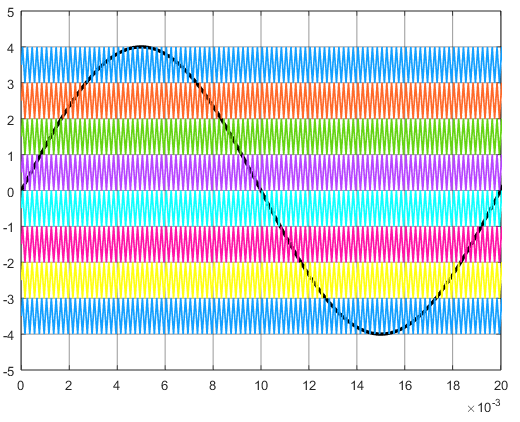
\includegraphics[width=16.5cm,height=10cm]{figures/PWMSCHEME.png}
	\end{center}
	\caption{Phase Disposition PWM Scheme}
	\label{PWM}
\end{figure}

Switching scheme used in this inverter is phase disposition pulse width modulation. Eight level-shifted triangular carrier signals are modulated using a single sine wave. All triangular waves are in phase. The amplitude of the sine wave is 4 units. Each triangular wave is level-shifted by 1 unit corresponding to each output level.\\

\begin{figure}[H]
	\begin{center}
		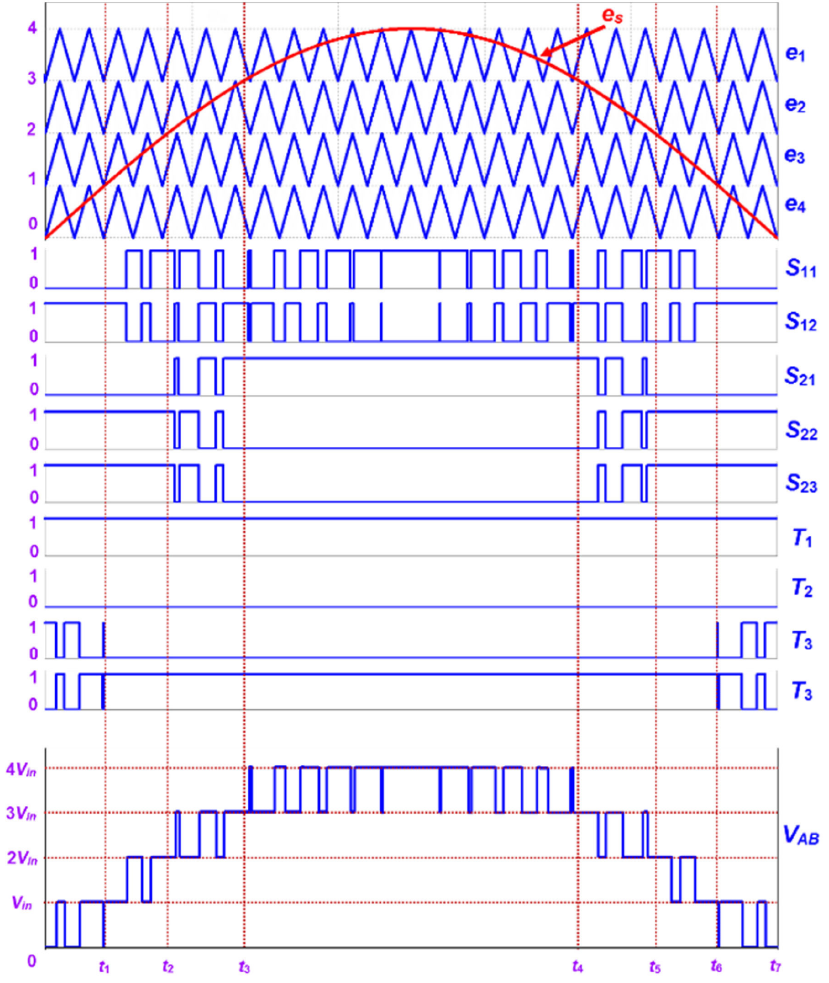
\includegraphics[width=15cm,height=16cm]{figures/switching_graph_states}
	\end{center}
	\caption{Switching diagram}
	\label{sc}
\end{figure} 

\clearpage

\chapter{SIMULATION RESULTS}

This chapter discusses about the simulation model of the nine level inverter based on switched capacitor structure. Further the analysis of the simulink model is also given.

\begin{figure}[h!]
\begin{center}
	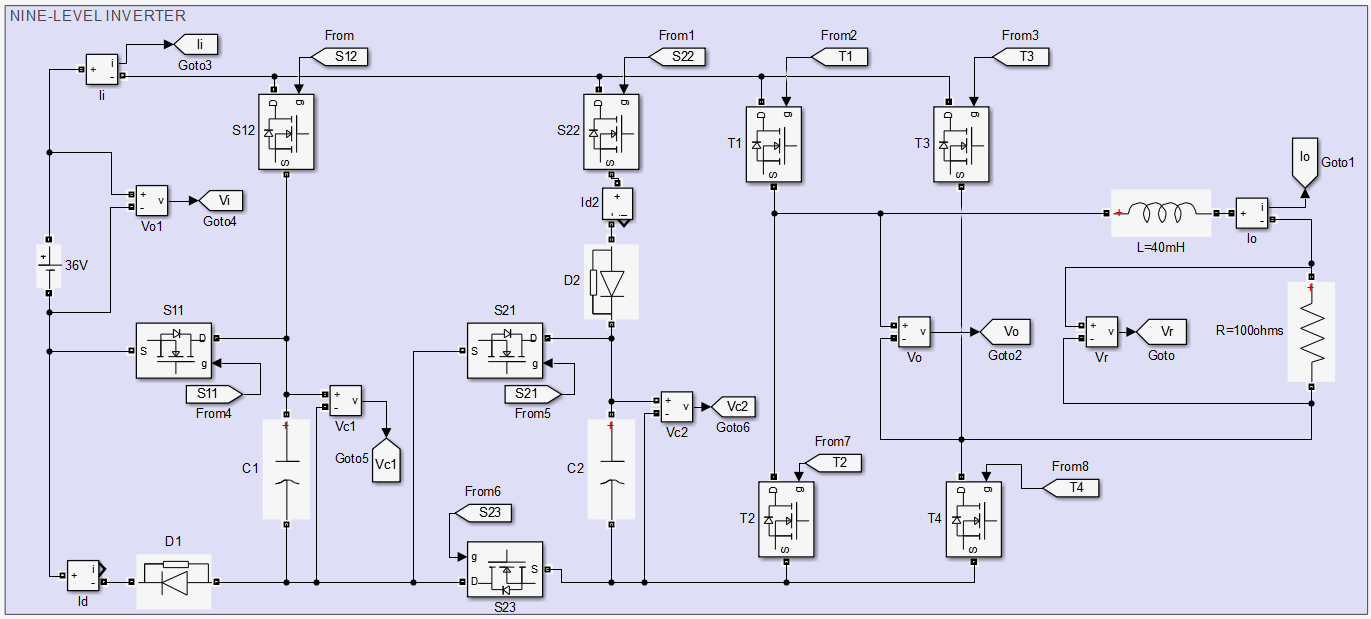
\includegraphics[width=16cm,height=8cm]{figures/SIMULINKCIRCUIT.png}
\end{center}
\caption{Simulink circuit}
\label{simlnk}
\end{figure}
The simulation of the NINE-LEVEL INVERTER was done using the simulink tool in matlab.
Operation of the inverter was verified with R and R-L load. Gating pulses are derived using PD-PWM technique. The switching delay and gate delay are neglected. The design consideration are given in the table below. \\

\begin{table}[H]
	\begin{center}
		\begin{tabular}{|c|c|} 
			\hline
			{\bf PARAMETER} & {\bf VALUE} \\  
			\hline
			$V_{in}$ & $36V$ \\ 
			\hline
			$V_{out}$ & $100V$ \\ 
			\hline
			Power Rating & $100W$ \\ 
			\hline
			$C_2$  & $2400{\mu}F$ , $180V$ \\
			\hline
			$C_2$  & $3600{\mu}F$ , $180V$ \\
			\hline
			Load($R+jX$) & $100 + j12$\\
			\hline
			Carrier frequency & $5000KH_z$  \\
			\hline
			Modulation & $50H_z$ \\
			\hline
			Switching scheme & PDPWM \\
			\hline
\end{tabular}
	\end{center}
	\caption{Simulation specification}
\end{table}

\begin{figure}[H]
	\begin{center}
		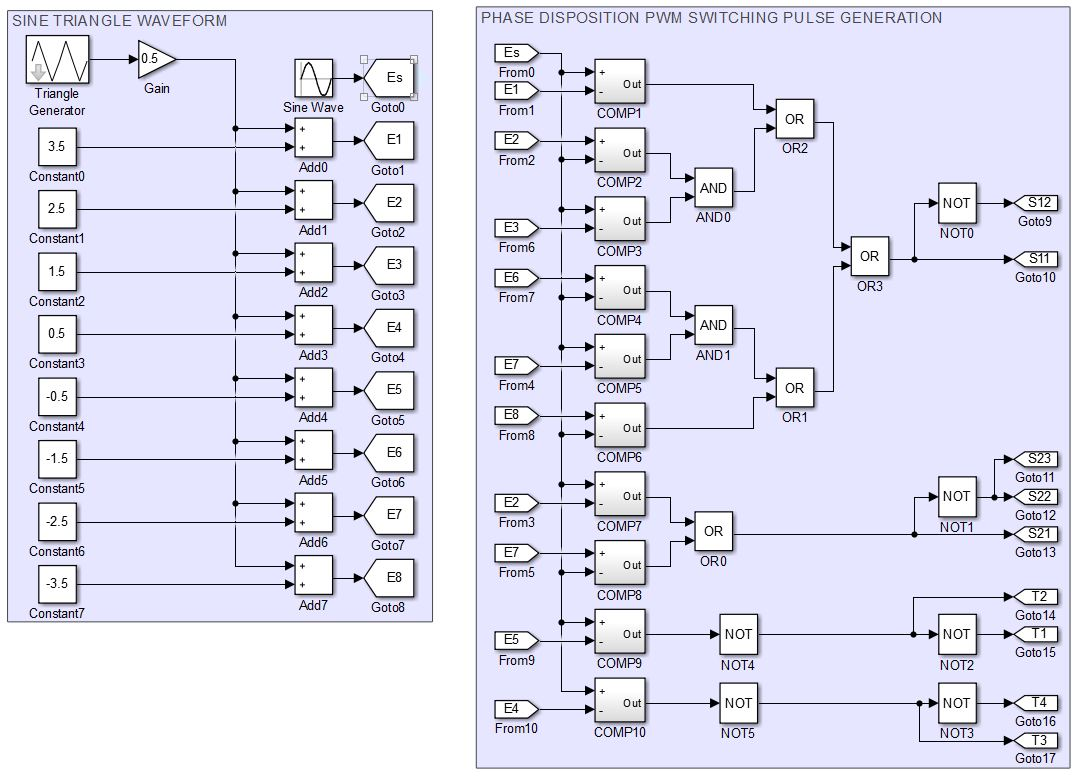
\includegraphics[width=15cm,height=12cm]{figures/PD_PWM.jpg}
	\end{center}
	\caption{Simulink Pulse Derivation}
	\label{PD_PWM}	
\end{figure}

\begin{figure}[H]
	\begin{center}
		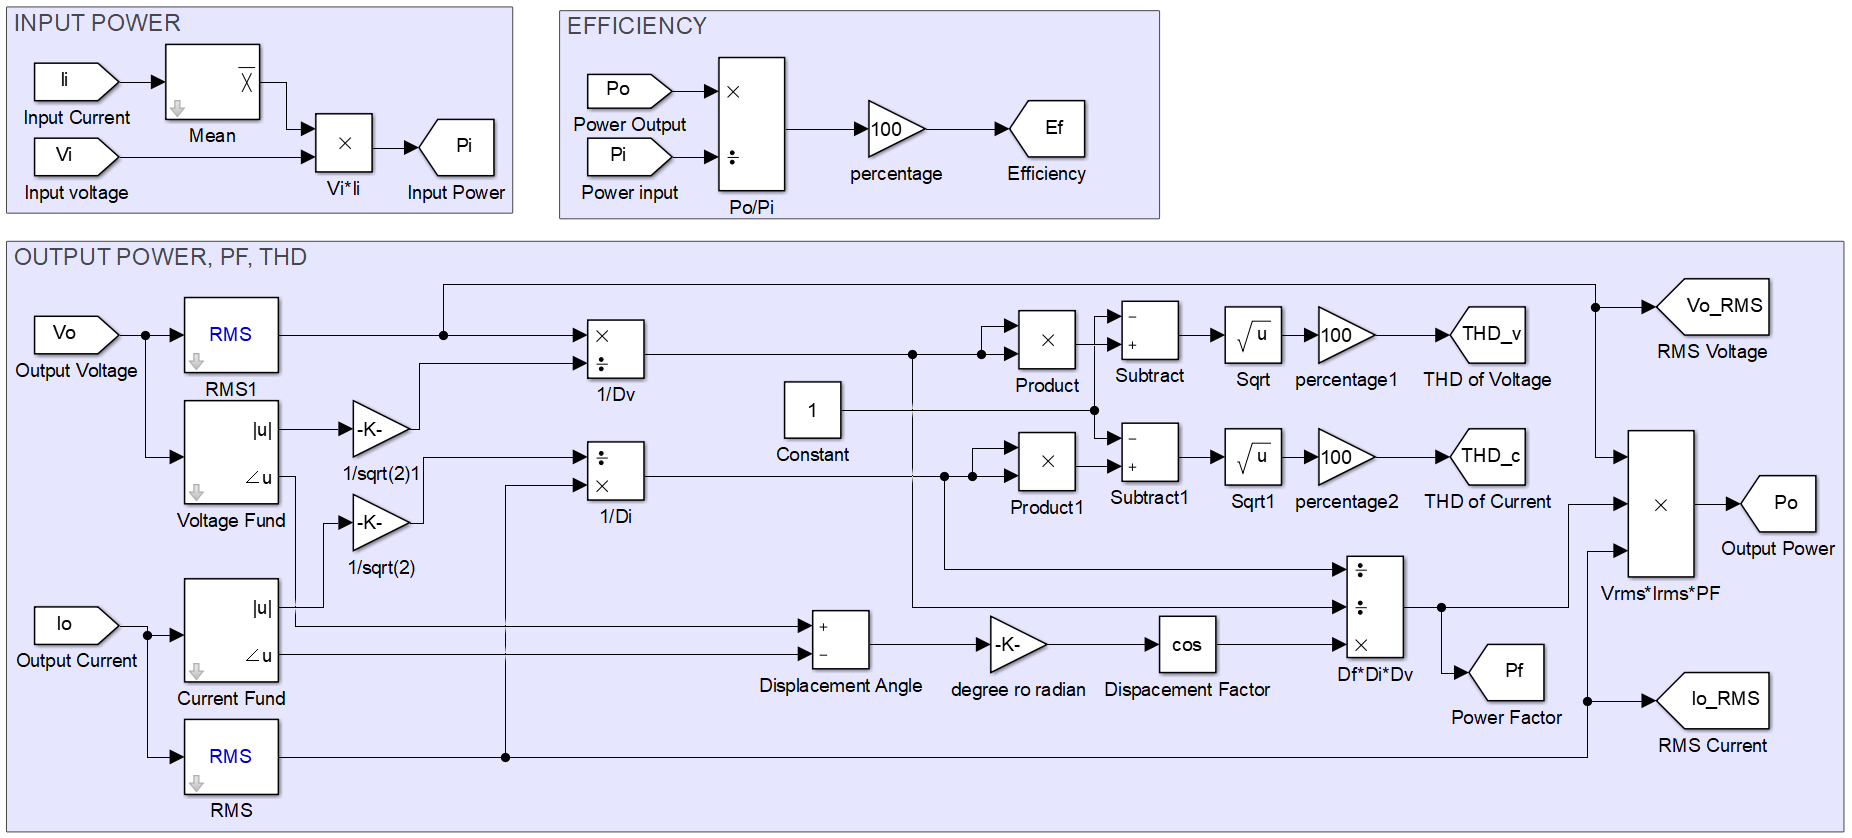
\includegraphics[width=15cm,height=8cm]{figures/Measurement.png}
	\end{center}
	\caption{Measurement Block}
	\label{measure}	
\end{figure}

\section{Result}
The output of the simulink simulation is shown in the following figures. Figure \ref{sout} shows the output voltage, capacitor voltage and current. Figure \ref{siman} shows the analyis after measurement of various inverter parameters. The peak voltage output of the inverter is $144V$. The RMS value of output voltage is $100V$. The RMS value of output current is $1A$. The capacitor voltage is nearly constant with neglegible ripple. The model is found to meet the expected design power outout of 100Watts.\\
\subsection{Peak Inverse Voltage(PIV)}
The voltag stress across the switches $S_{11}$ and $S_{12}$ are $V_{in}$ where $V_{in}$ is the input dc voltage. The voltage stress across the switches $S_{21}$, $S_{22}$ and $S_{23}$ are $2V_{in}$. The voltage stress across the switches of H-bridge $T_1$, $T_2$, $T_3$ and $T_4$ are $4V_{in}$. The peak load voltage is $4V_{in}$.\\
\subsection{Total Harmonic Distortion(THD)}
The output voltage waveform for a load resistance of $Z_L = 100\Omega$ and its FFT analysis is shown in figure \ref{FFT1}. It's THD is found to be 13.92\%. The output voltage waveform for a load resistance of $Z_L = 100\Omega + j12\Omega$ and its FFT analysis is shown in figure \ref{FFT2}. It's THD is found to be 1.013\%.\\
\subsection{Efficiency}
Efficiency of the switched capacitor nine-level inverter for a load of $Z_L = 100\Omega + j12\Omega$ is found to be 95.37\% for a power output of $100W$.\\
\begin{figure}[H]
	\begin{center}
		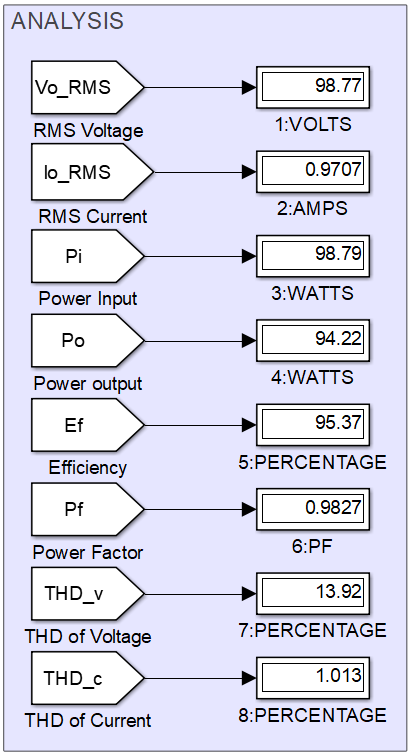
\includegraphics[width=7cm,height=12cm]{figures/SIMULINKANALYSIS.png}
	\end{center}
	\caption{Simulink analysis}
	\label{siman}
\end{figure}
\begin{figure}[H]
	\begin{center}
		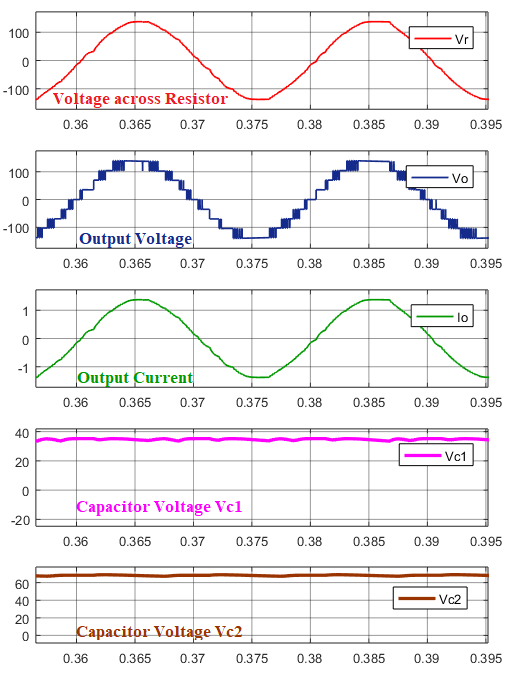
\includegraphics[width=15cm,height=20cm]{figures/SIMULINKOUTPUT.png}
	\end{center}
	\caption{Simulink Output}
	\label{sout}	
\end{figure}
\begin{figure}[H]
	\begin{center}
		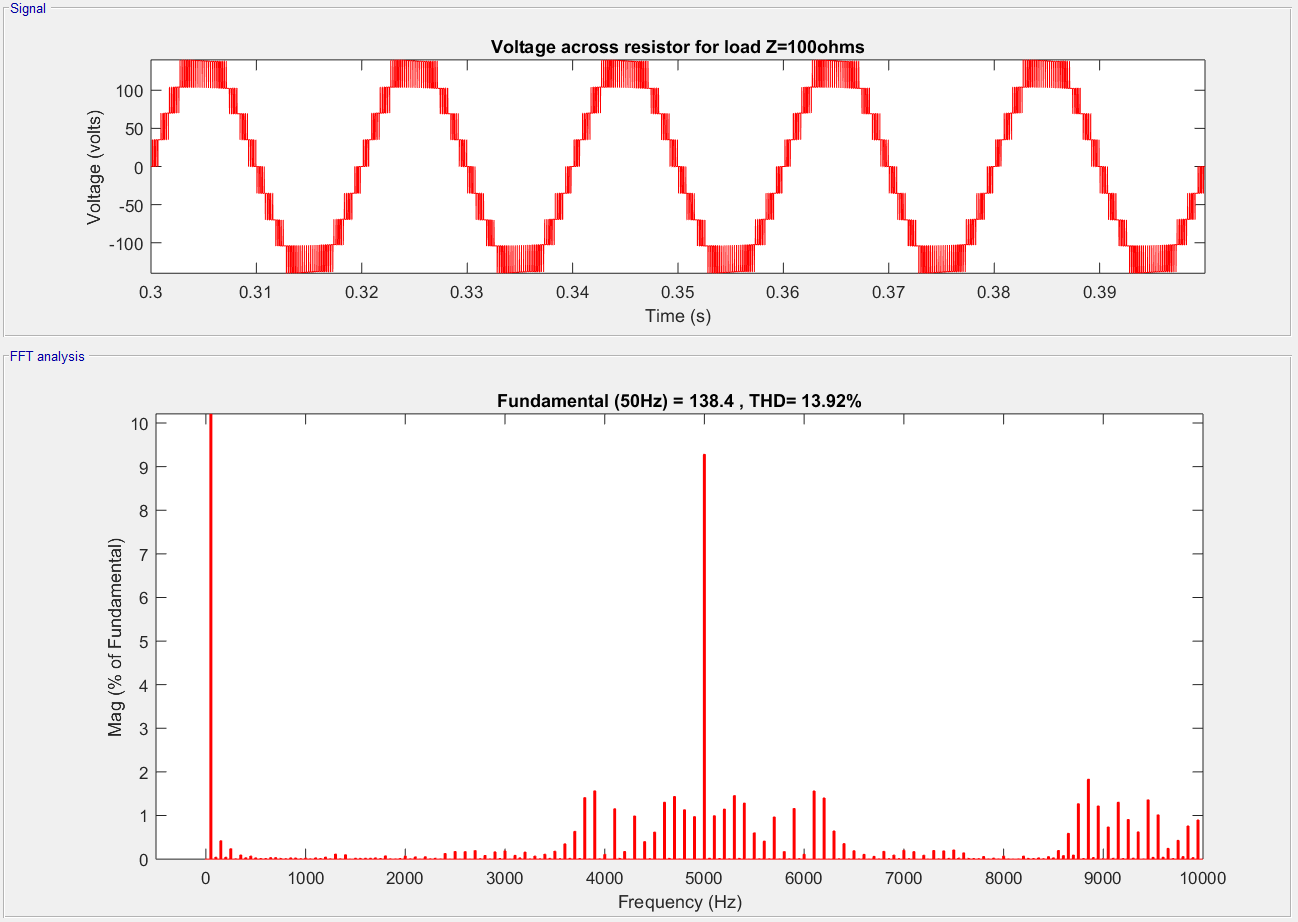
\includegraphics[width=14cm,height=8.5cm]{figures/FFT_Ronly.png}
	\end{center}
	\caption{Simulink FFT analysis with R load}
	\label{FFT1}
\end{figure}
\begin{figure}[H]
	\begin{center}
		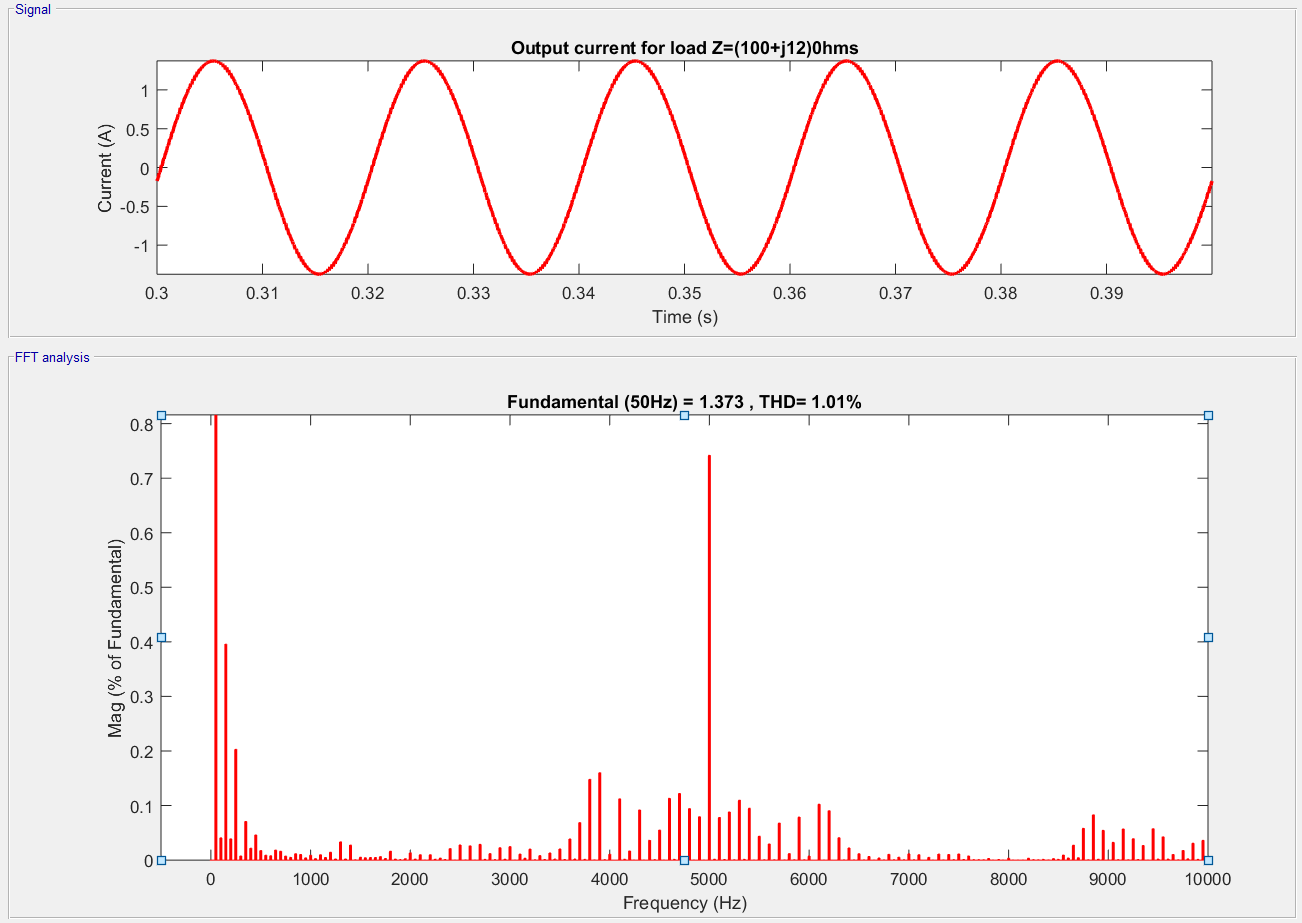
\includegraphics[width=14cm,height=8.5cm]{figures/FFT_RL.png}
	\end{center}
	\caption{Simulink FFT analysis with RL load}
	\label{FFT2}
\end{figure}


\clearpage

\chapter{HARDWARE IMPLEMENTATION AND RESULTS}

This chapter discusses in detail about the hardware implementation of the nine livel inverter based on switched capacitor structure. The components used in realization are expalined in detail. Various stages of the work like PCB realization etc are also included. The following table summarises the hardware specifications of the project.\\

\begin{table}[h!]
	\begin{center}
	\begin{tabular}{|c|c|} 
		\hline
		{\bf PARAMETER} & {\bf VALUE} \\  
		\hline
		$V_{in}$ & $36V$ \\ 
		\hline
		$V_{out}$ & $100V$ \\ 
		\hline
		Power Rating & $100W$ \\ 
		\hline
		Switch Used & MOSFET IRFP460 \\ 
		\hline
		Diode & MUR460\\
		\hline
		MOSFET Drives & TLP250 \\ 
		\hline
		$C_2$  & $2400{\mu}F$ , $180V$ \\
		\hline
		$C_2$  & $3600{\mu}F$ , $180V$ \\
		\hline
		Carrier frequency & $5000KH_z$  \\
		\hline
		Modulation & $50H_z$ \\
		\hline
		Switching scheme & PDPWM \\
		\hline
		Switching pulse realisation & DSPIC30F2020\\
		\hline
		\end{tabular}
		\end{center}
	
	\caption{Hardware specification}
	\end{table}
	\vspace{1.0cm}
	\section{MOSFET IRFP460}	
	Third Generation HEXFETs from international Rectifier provide the designer with the best combination of fast switching ruggedized device design, low on-resistance and cost-effectiveness. The TO-247 package is preferred for commercial industrial applications where high power levels preclude the use of TO-220 devices. It also provides greater creepage between pins to meet the requirements of most safety specifications. \\
	\begin{minipage}{10cm}
		\begin{figure}[H]
			\begin{center}
				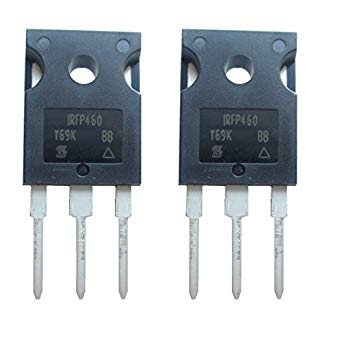
\includegraphics[width=4cm,height=4cm]{figures/IRFP460.jpg}
			\end{center}
			\caption{IRFP460}
		\end{figure}
	\end{minipage}
	\begin{minipage}{5cm}
		\begin{table}[H]
			\begin{center}
				\begin{tabular}{|c|c|} 
					\hline
					$V_{DSS}$ & $500V$\\ 
					\hline
					$V_{GS}$ & $2-4V$ \\ 
					\hline
					$R_{DS(on)}$ & $0.27ohm$\\
					\hline
					$t_{d(on)}$& $18ns$ \\ 
					\hline					
					$t_{d(off)}$  & $110ns$ \\
					\hline
					$I_{s}$  & $20A$  \\
					\hline
				\end{tabular}
			\end{center}
			\caption{IRFP460 Specs}
		\end{table}
	\end{minipage}	
	\section{MUR460}
		MUR460 is designed for use in switching power supplies, inverters and as free-wheeling diodes. These devices have the following features:\\
	\begin{minipage}{10cm}
		\begin{table}[H]
			\begin{center}
				\begin{tabular}{|c|c|} 
					\hline
					Peak Reverse Voltage & $600V$\\ 
					\hline
					Average Forward Current & $4A$\\ 
					\hline
					Reverse Recovery Time & $75nS$\\
					\hline
					Forward Recovery Time & $50nS$\\
					\hline
				\end{tabular}
			\end{center}
			\caption{MUR460 Specs}
		\end{table}
	\end{minipage}
	\begin{minipage}{5cm}
		\begin{figure}[H]
			\begin{center}
				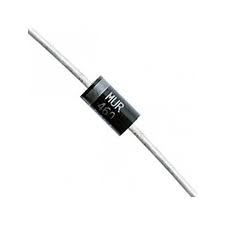
\includegraphics[width=4cm,height=4cm]{figures/MUR460.jpg}
			\end{center}
			\caption{MUR460}	
		\end{figure}		
	\end{minipage}\\

\noindent1. 175 $^{\circ}$ C operating juction temperature \\
	3. Low forward voltage \\
	4. Low leakage current\\
	5. High temperature glass passivated junction\\
	
\section{DSPIC30F2020}
\begin{figure}[h!]
\begin{center}
	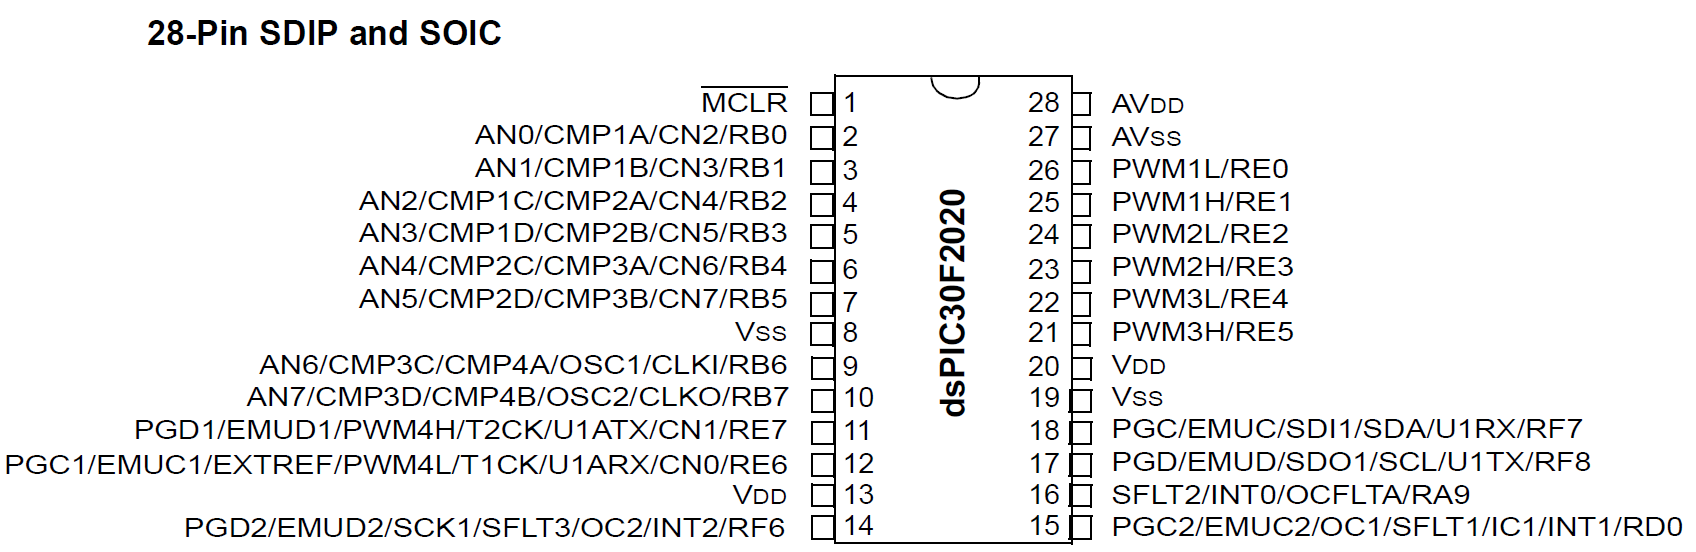
\includegraphics[width=16cm,height=6cm]{figures/dsp_PINOUT.png}
\end{center}
\caption{DSPICIC30F2020 Pin diagram.}
	
\end{figure}


High-Performance Modified RISC CPU:\\

\begin{itemize}

\item • Modified Harvard architecture
\item• C compiler optimized instruction set architecture
\item• 83 base instructions with flexible addressing modes.
\item• 24-bit wide instructions, 16-bit wide data path
\item• 12 Kbytes on-chip Flash program space
\item• 512 bytes on-chip data RAM
\item• 16 x 16-bit working register array.
\item• Up to 30 MIPS operation:\\
- Dual Internal RC\\
- 9.7 and 14.55 MHz \\
- 6.4 and 9.7 MHz \\
- 32X PLL with 480 MHz VCO\\
- PLL inputs \\
- External EC clock 6.0 to 14.55 MHz\\
- HS Crystal mode 6.0 to 14.55 MHz\\
\item• 32 interrupt sources
\item• Three external interrupt source
\item• 8 user-selectable priority levels for each interrupt.
\item• 4 processor exceptions and software traps.
\end{itemize}
 
 \vspace{0.7cm}
{\bf Power Supply PWM Module Features:}
 \begin{itemize}
 	
 	\item • Four PWM generators with 8 outputs
 	\item • Each PWM generator has independent time base
 	and duty cycle
 	\item • Duty cycle resolution of 1.1 ns at 30 MIPS
 	\item • Individual dead time for each PWM generator:\\
 	- Dead-time resolution 4.2 ns at 30 MIPS\\
 	- Dead time for rising and falling edges
 	\item • Phase-shift resolution of 4.2 ns @ 30 MIPS
 	\item • Frequency resolution of 8.4 ns @ 30 MIPS
 	\item • PWM modes supported:
 	- Complementary\\
 	- Push-Pull\\
 	- Multi-Phase\\
 	- Variable Phase\\
 	- Current Reset\\
 	- Current-Limit
 	\item • Independent Current-Limit and Fault Inputs
 	\item • Output Override Control
 	\item • Special Event Trigger
 	\item • PWM generated ADC Trigger
 \end{itemize}

DSPIC30F2020 is programmed so as to produce driving signals to the switches in the inverter circuit. The DSPIC30F2020 also has PWM capabilities which can be operated by giving basic values like the duty cycle.

\section{Gate Driver Opto Coupler}
The TLP250 consists of a GaAlAs light emitting diode and an integrated photo detector. The unit is an 8-lead DIP package. TLP250 is suitable for gate-driving circuit of IGBT or power MOSFET. \\

\noindent\begin{minipage}{9cm}
	\begin{table}[H]
		\begin{center}
			\begin{tabular}{|c|c|} 
				\hline
				Input Threshold current & $5mA$\\ 
				\hline
				Input Reverse Voltage & $5V$\\ 
				\hline
				Operating frequency & $25KHz$\\ 
				\hline
				Junction Temperature & $125^{\circ}C$\\ 
				\hline
				Isolation Voltage & $2500V$\\ 
				\hline
				Supply Current & $11mA$\\ 
				\hline
				Supply Voltage & $10V-35V$\\
				\hline
				Output Current & $1.5A$\\
				\hline
				Switching time & $1.5\mu S$\\
				\hline
			\end{tabular}
		\end{center}
		\caption{TLP250 Specs}
	\end{table}
\end{minipage}
\begin{minipage}{5cm}
	\begin{figure}[H]
		\begin{center}
			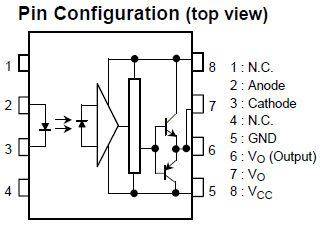
\includegraphics[width=7cm,height=5cm]{figures/tlp.png}
		\end{center}
		\caption{TLP250 Pin Configuration}
	\end{figure}
\end{minipage}\\ \vspace{0.1in}

The TLP250 plays an important role in the inverter circuit. It is used to produce high-voltage pulses as supplied to it such that the input pulse is electrically isolated from the output. The input section consists of an LED. The gate pulse of 5V is dropped to the LED driving voltage using a resistor. The output stage consists of a photo detector and transistors in totem-pole structure. When a gate pulse is supplied to the input stage, the LED is illuminated in the ON stage and otherwise in the OFF stage. This produces corresponding pulse signal in the output using the photo detector of amplitude equal to the gate drive power supply which in this case is 15V.\\

\section{Gate Power Supply}

The 15 V pulse is necessary to drive IRFP460 since the output voltage from the DSPIC is insufficient to drive the high power switch. The 15 V pulse is obtained using the Gate driver optocoupler which requires a voltage input of 15V called Gate Driver Power Supply. The Gate driver power supply circuit consists of 10 output configurations consisting of a transformer, regulator configuration. The driving circuit is fired using the gate pulse. The transformer is wound with 46 turns in the primary and 37 in the secondary so that an input signal of 24 Volt can be transformed into 20 V.\\

\begin{figure}[H]
	\begin{center}
		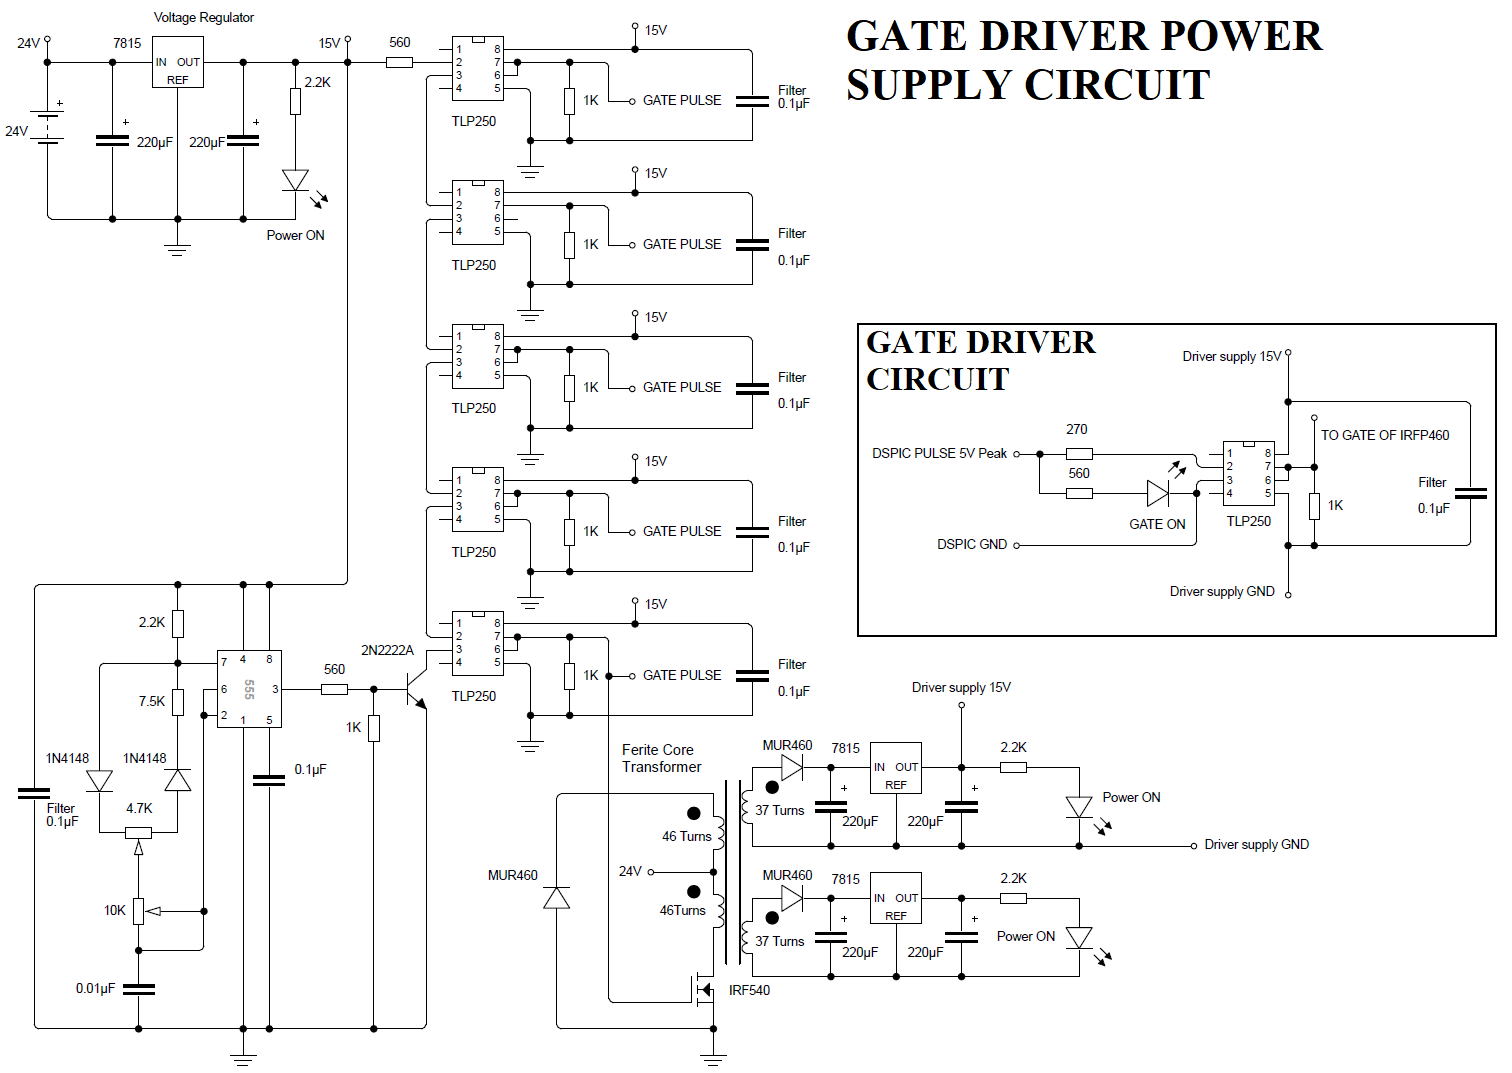
\includegraphics[width=16cm,height=11cm]{figures/overall.png}
	\end{center}
	\caption{Gate Driver Power Supply Circuit}
\end{figure}

 When the pulse is high, the IRF540 is ON. Hence, the voltage of 24 Volt is induced on both the primaries of the transformer. A voltage almost equal to 20V is then induced on the secondary windings according to dot convention. This signal is then filtered, regulated to 15 V and filtered once again to produce the supply. In the OFF state of the IRF540, the presence of the MUR460 diode allows the flow of the remaining energy stored back to the supply, thus completing the circuit. Ten similar configurations produce 10 sources of 15 V each which are isolated from each other. Out of these, 9 sources are used to drive the TLP250 in the inverter circuit whereas one of them is used to drive the DSPIC. The gate pulse to drive the IRF540 switch is obtained by using a 555 IC timer network. The IC network is so designed that adjusting the 10k pot helps to vary the duty cycle and the 4.7k pot can be used to vary the time period and thereby frequency.\\

\section{PCB Realization}

\begin{minipage}{8cm}
	\begin{figure}[H]
		\begin{center}
			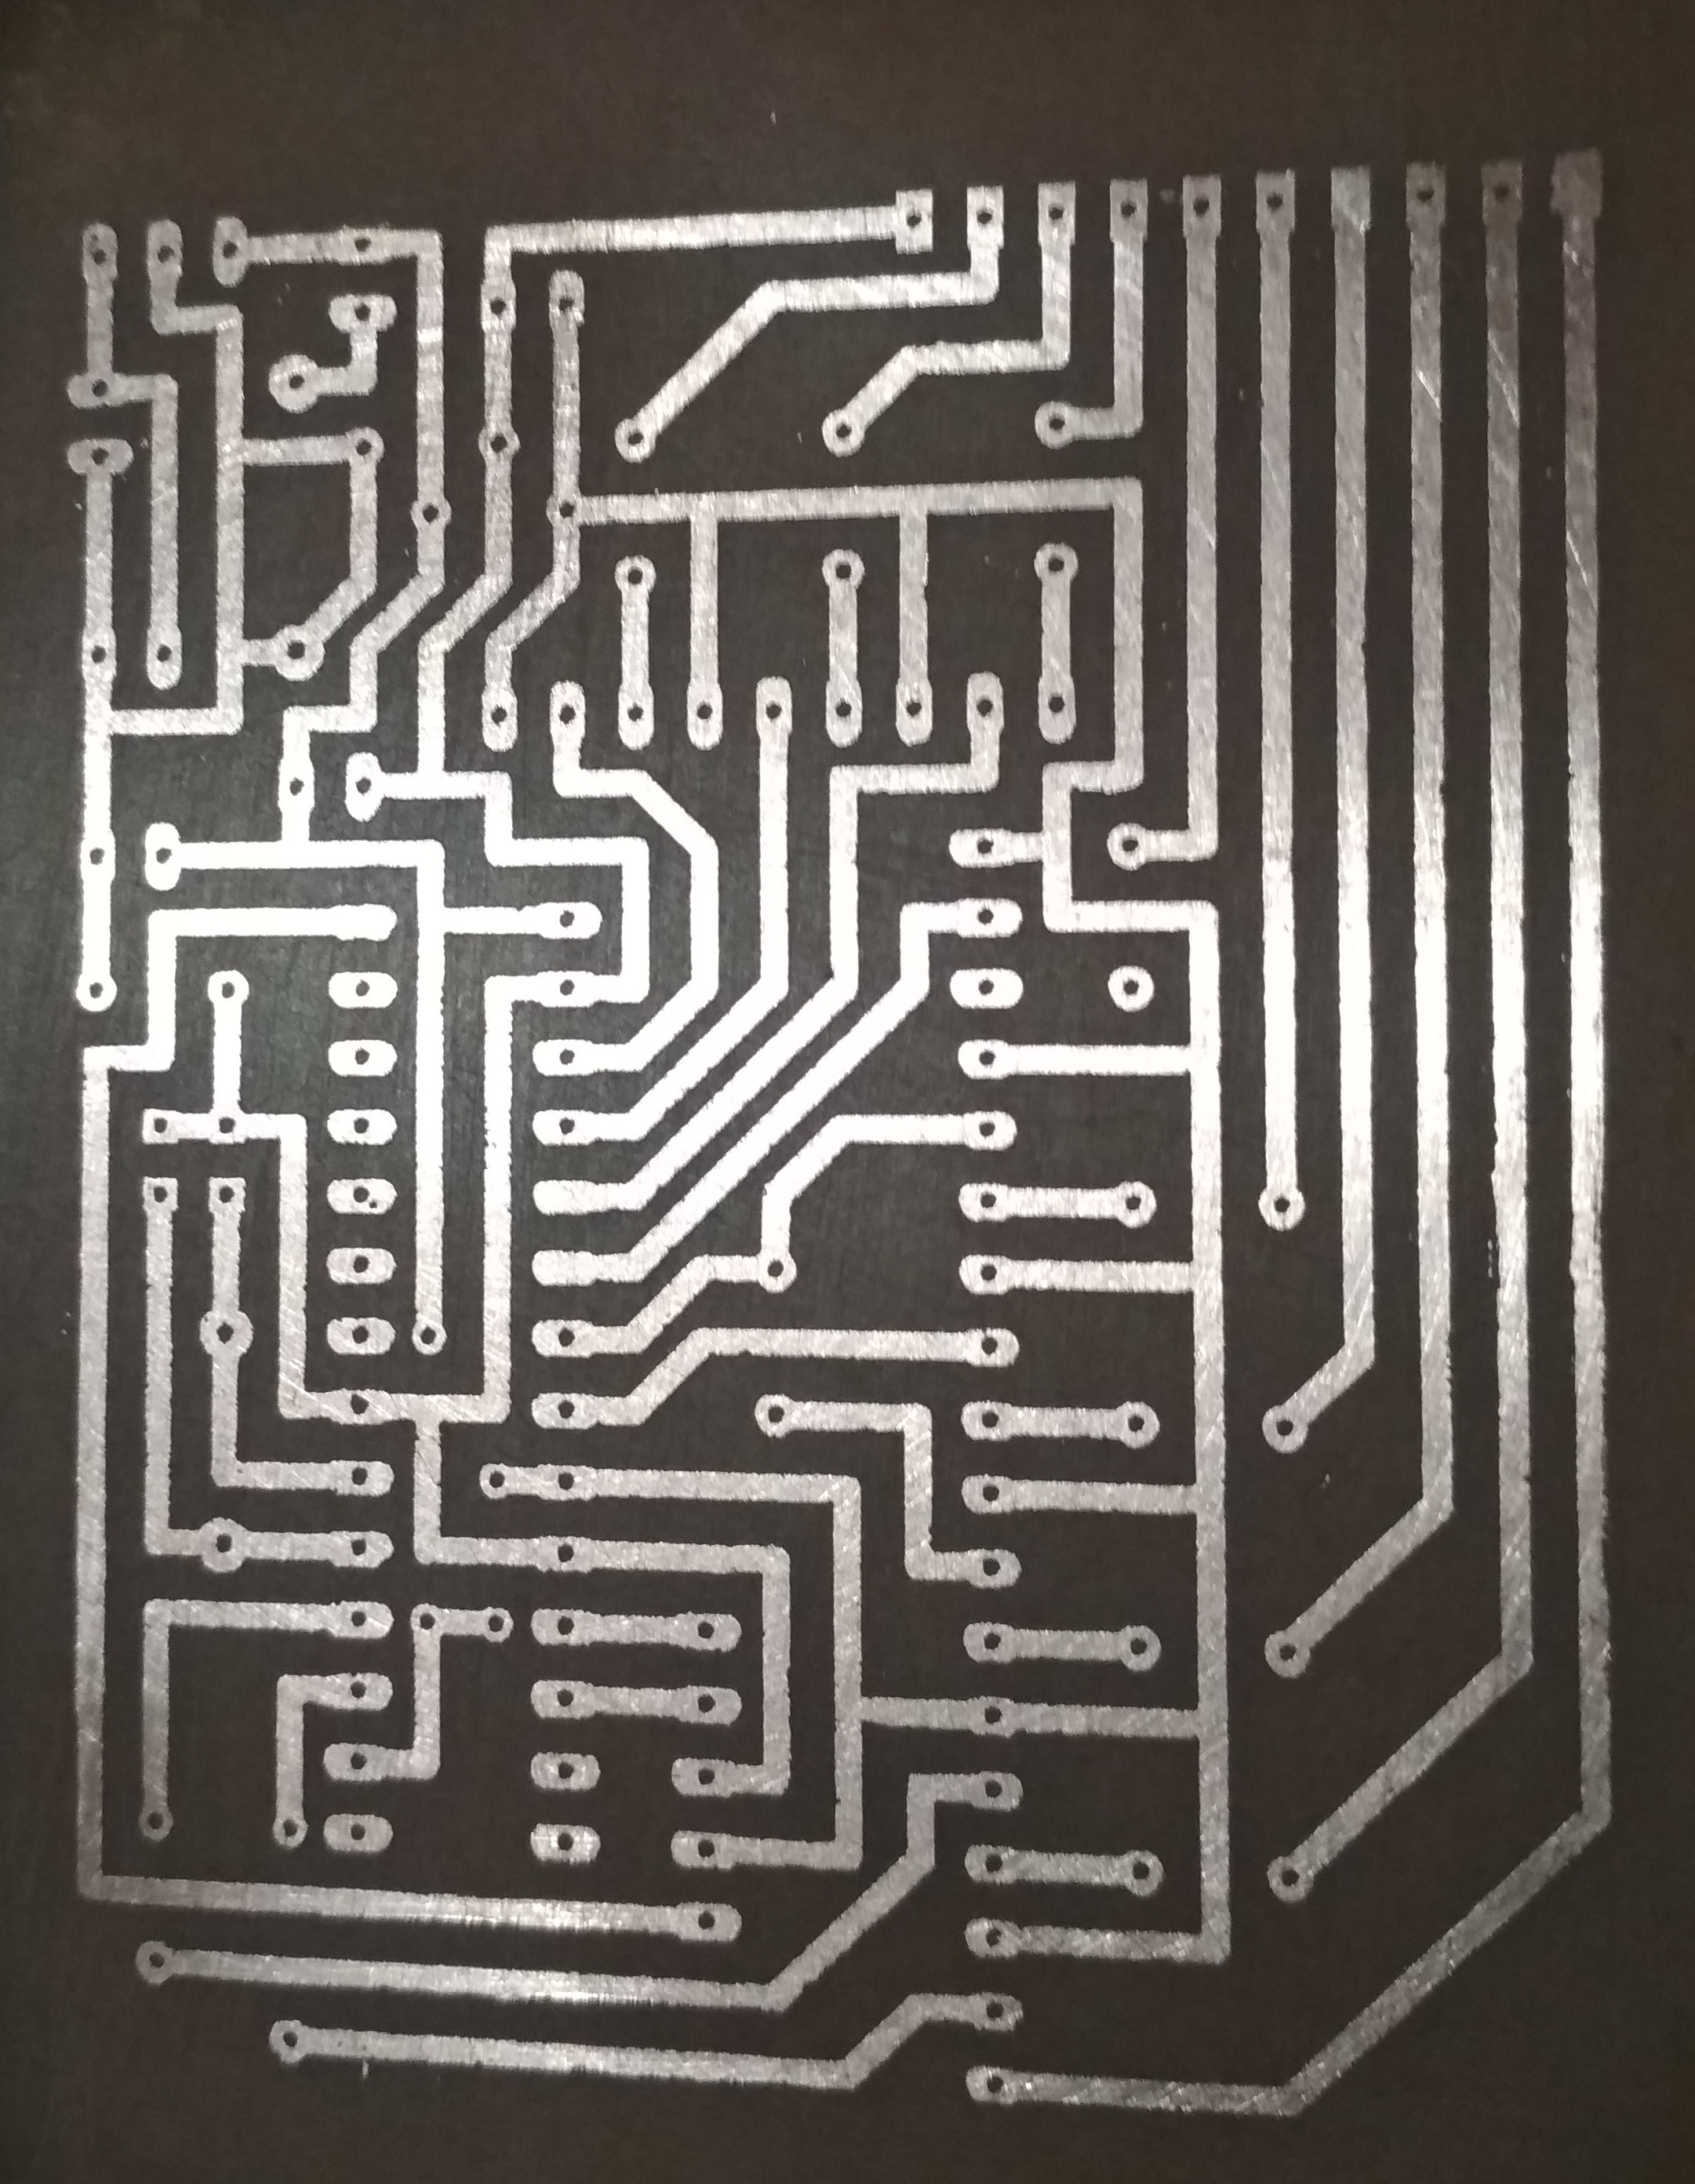
\includegraphics[width=7cm,height=10cm]{figures/dsp1.png}
		\end{center}
			\caption{DSPIC Board Design}\label{DSP}
	\end{figure}
\end{minipage}
\begin{minipage}{8cm}
	\begin{figure}[H]
		\begin{center}
			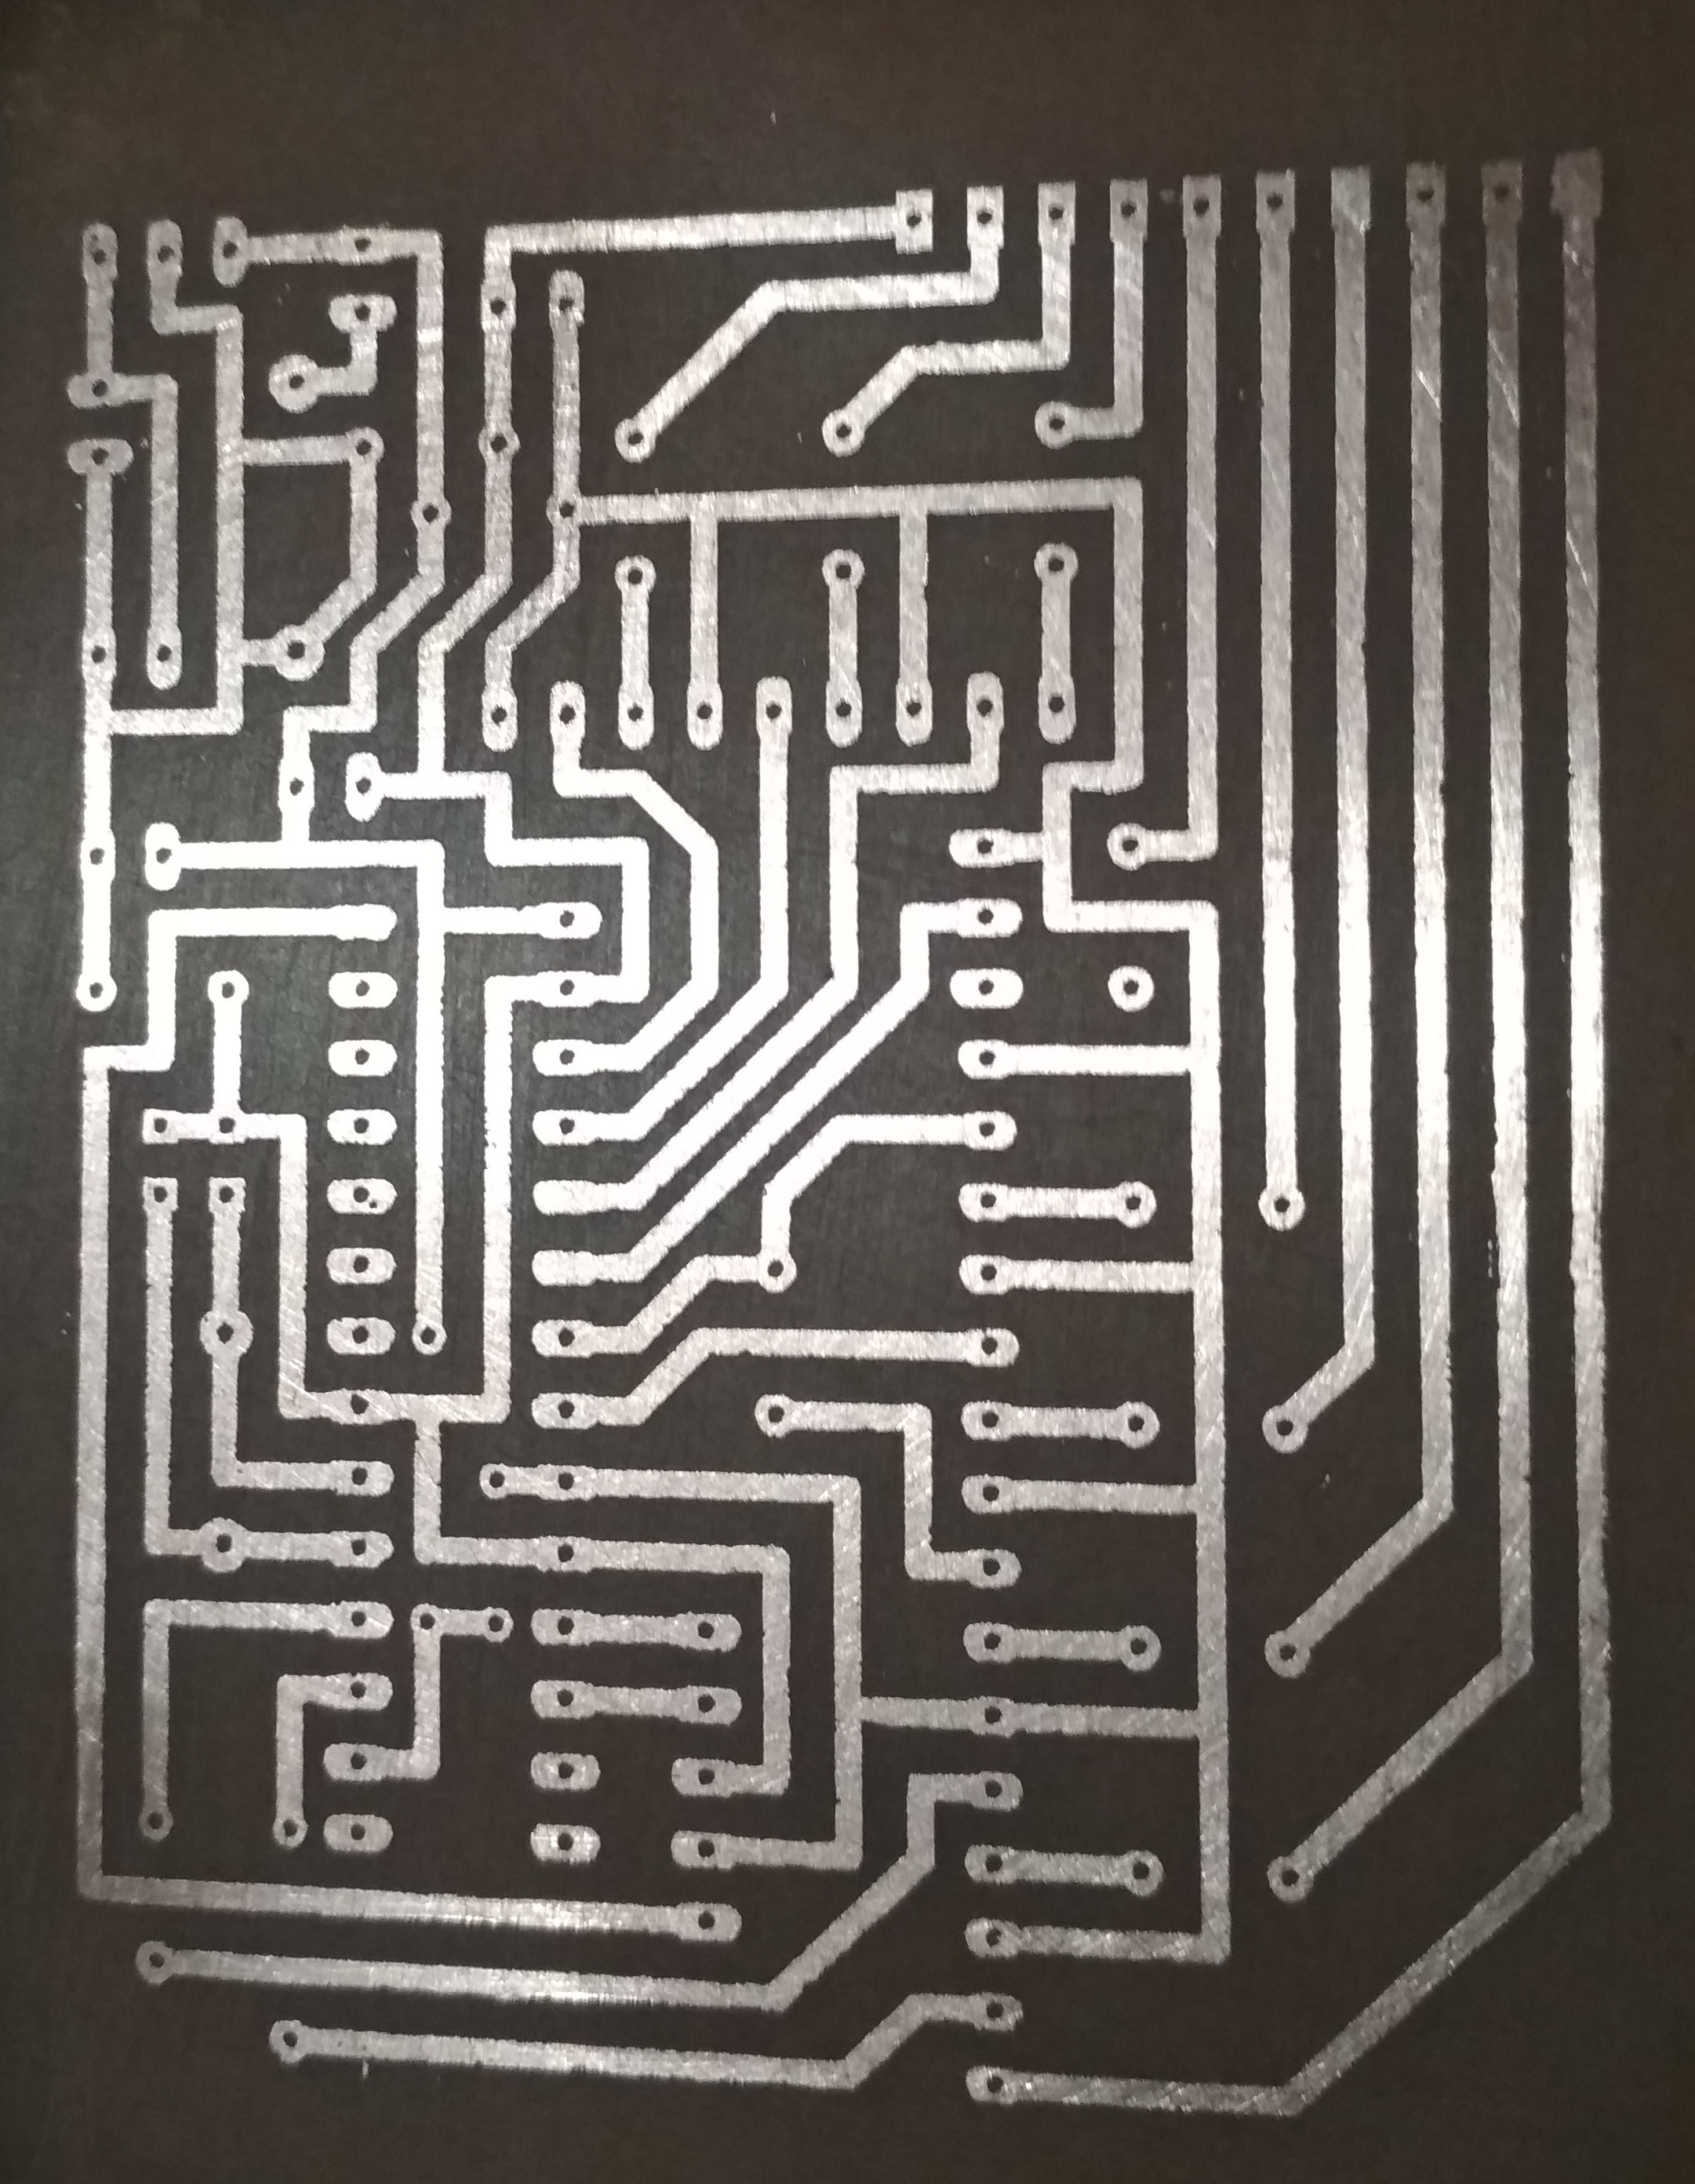
\includegraphics[width=7cm,height=10cm]{figures/dsp1.jpg}
		\end{center}
			\caption{DSPIC Board PCB Realisation}\label{DSP1}
	\end{figure}
\end{minipage}

\noindent\begin{minipage}{5.3cm}
	\begin{figure}[H]
		\begin{center}
			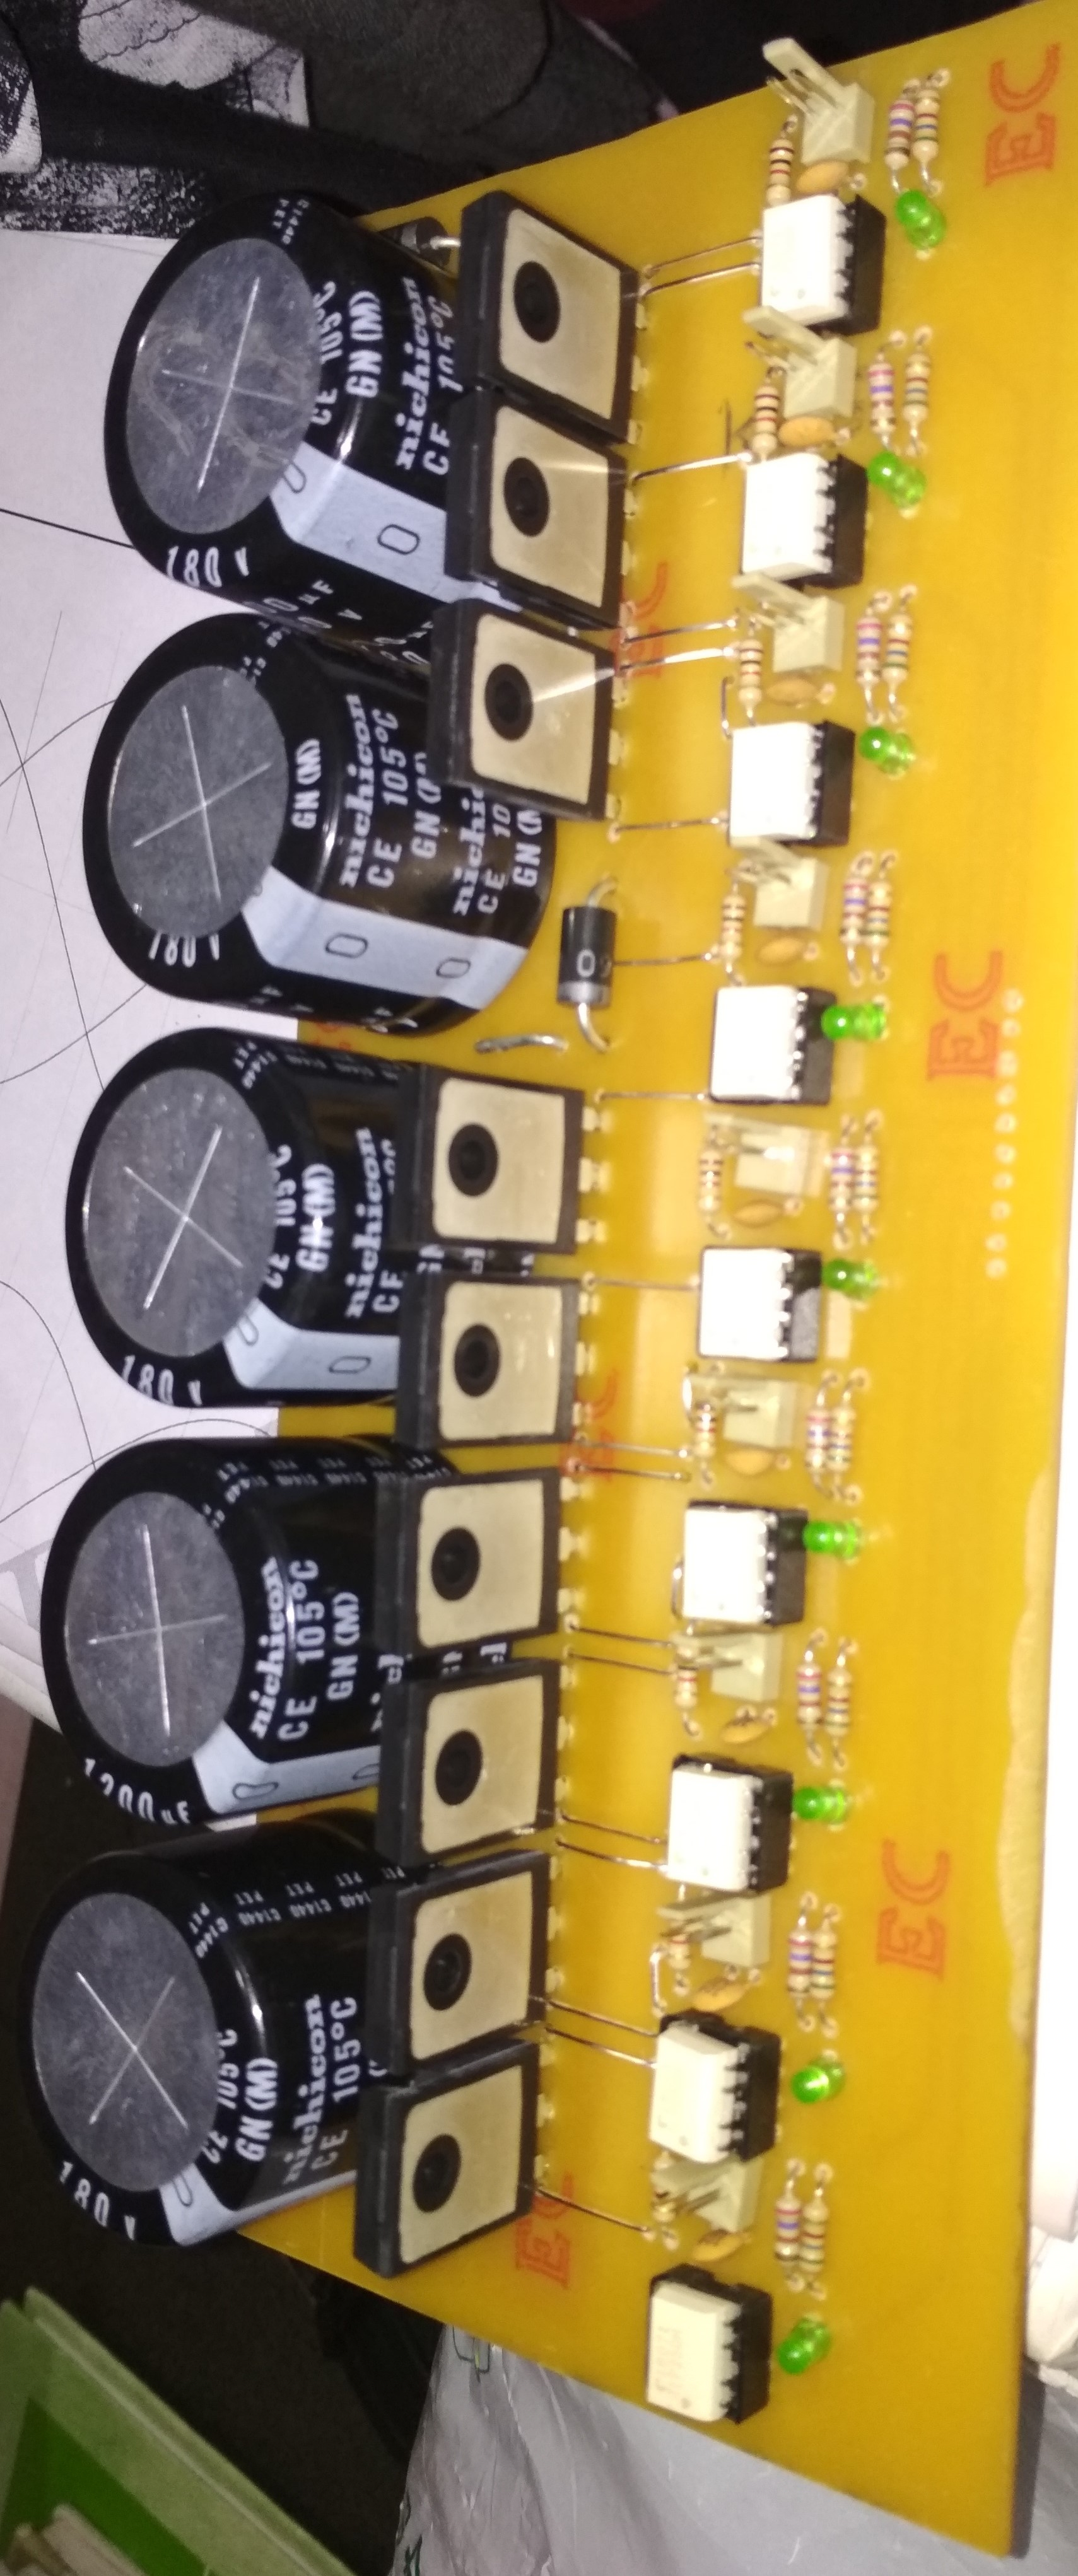
\includegraphics[width=4.5cm,height=8cm]{figures/inverter_art.jpg}
		\end{center}
		\caption{Inverter Realisation}\label{DSPQ}
	\end{figure}
\end{minipage}
\begin{minipage}{5.3cm}
	\begin{figure}[H]
		\begin{center}
			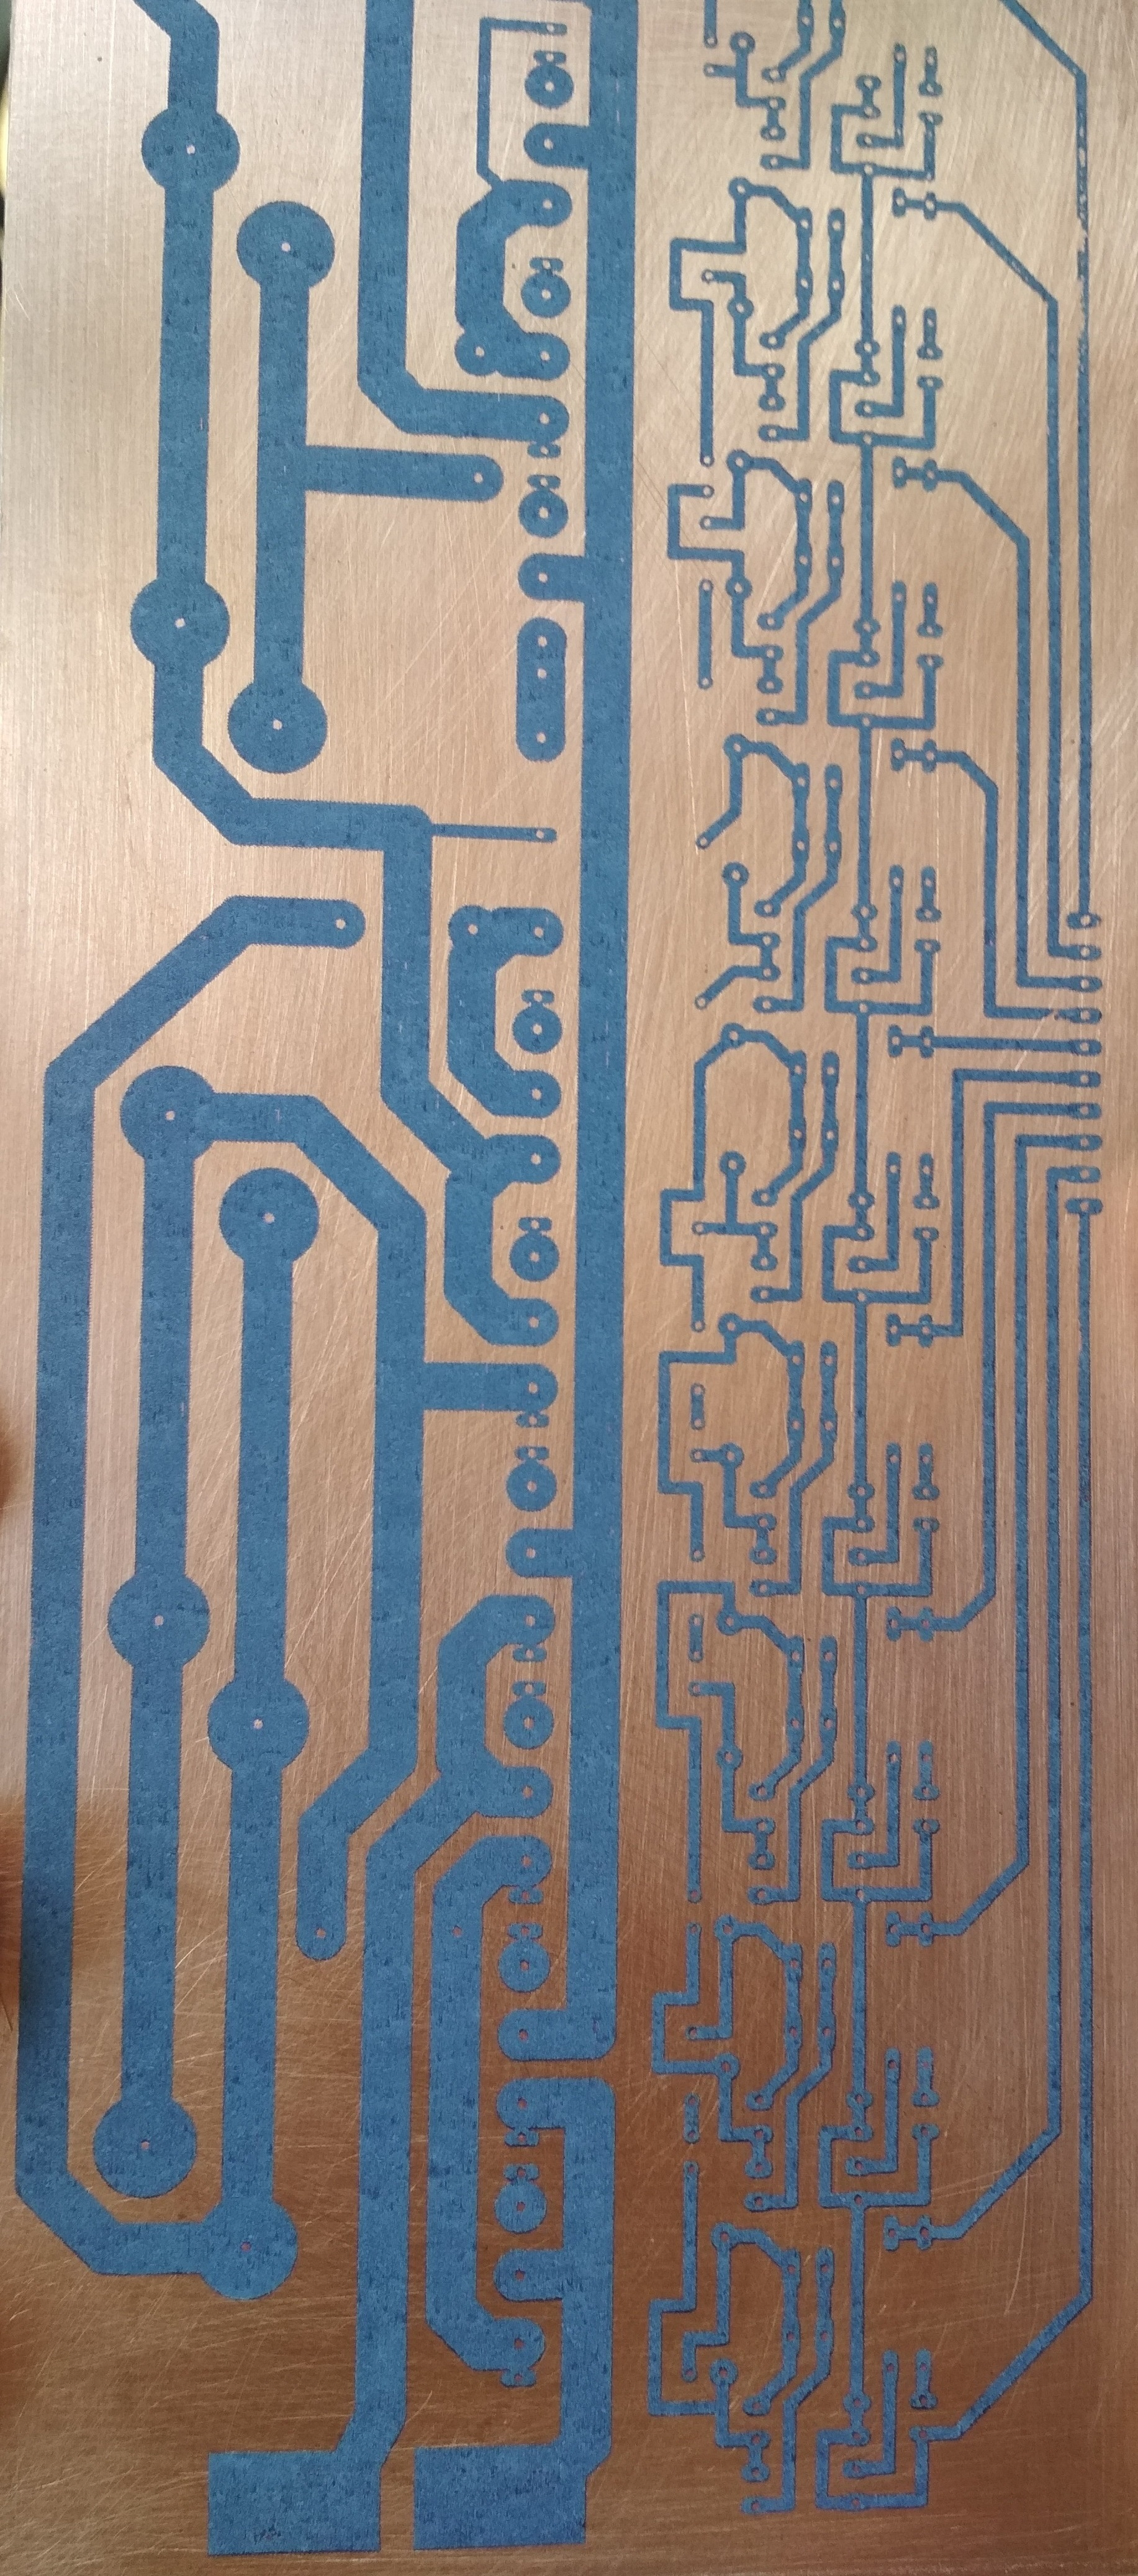
\includegraphics[width=4.5cm,height=8cm]{figures/invertert.jpg}
		\end{center}
		\caption{PCB Toner Transfer}\label{DSPW}
	\end{figure}
\end{minipage}
\begin{minipage}{5.3cm}
	\begin{figure}[H]
		\begin{center}
 			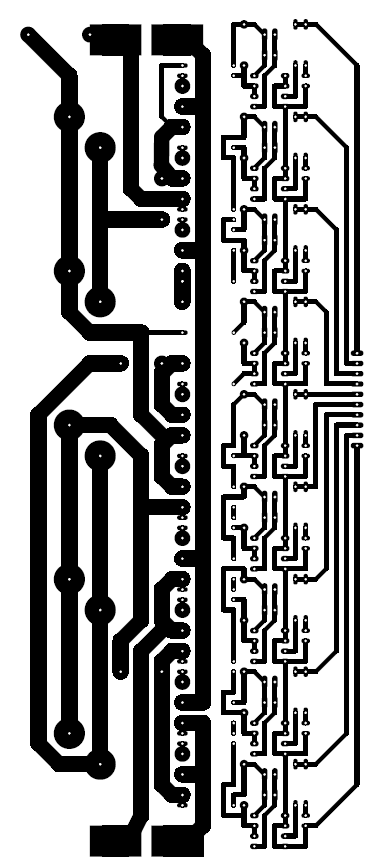
\includegraphics[width=4.5cm,height=8cm]{figures/INVERTERB.PNG}
 		\end{center}
 		\caption{Inverter PCB Design}\label{DSPE}
 	\end{figure}
\end{minipage}\vspace{0.5in}\\

All the required circuits are etched on a copper plate by displacement method using $FeCl_3$ solution. This involves marking the tracks on the copper plate using either toner transfer method which involves the transfer of printed ink on glossy paper into the copper plate. This plate is then placed in a $FeCl_3$ bath and agitated till the Cu from the non-painted region is eroded. This produces proper Cu tracks on the board. Necessary holes are pierced on the board so that necessary elements can be fixed on the same.\\

\noindent\begin{minipage}{8cm}
	\begin{figure}[H]
		\begin{center}
			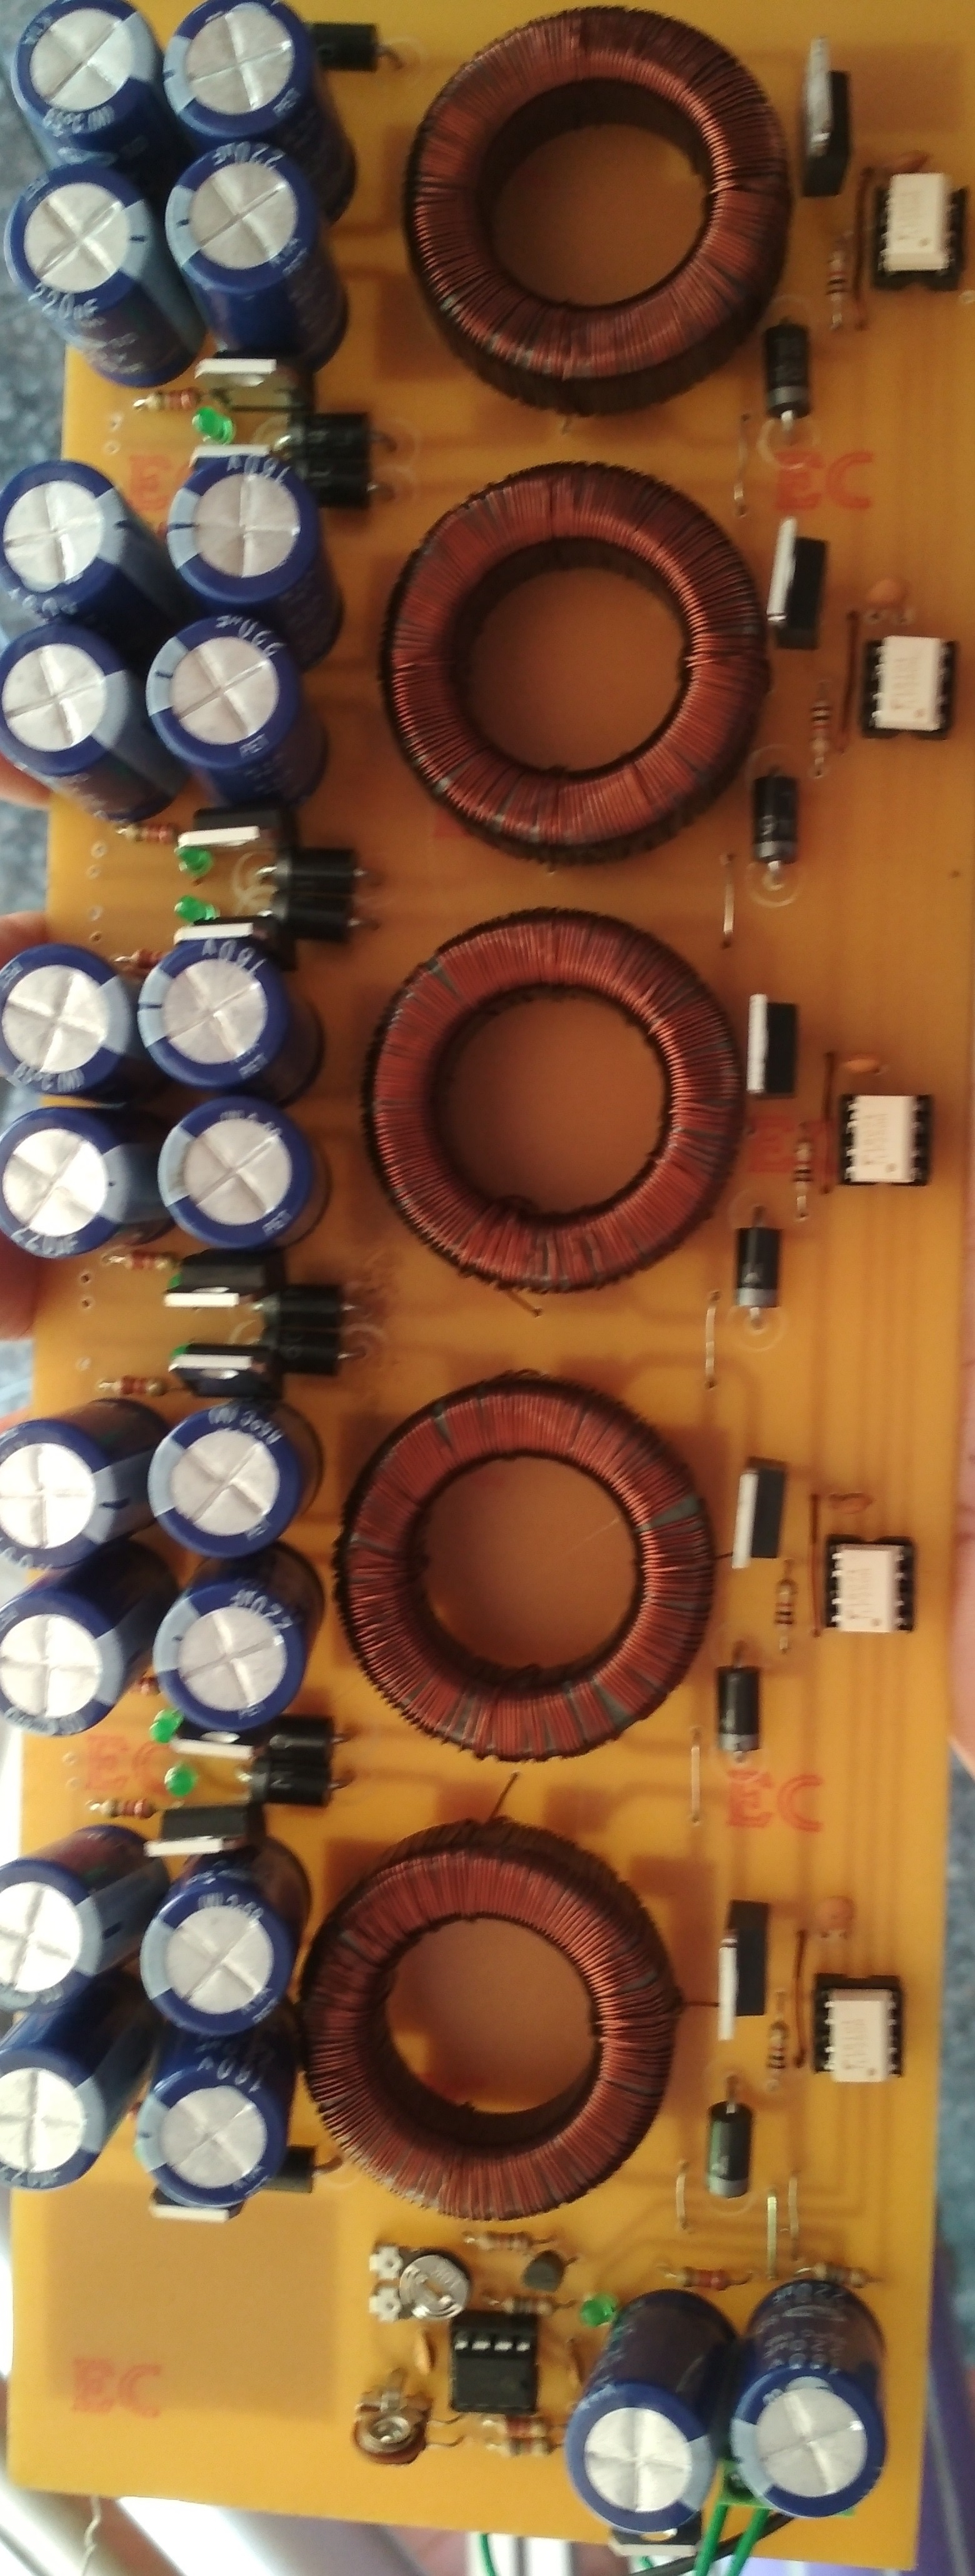
\includegraphics[width=8cm,height=18cm]{figures/driver.jpg}
		\end{center}
			\caption{Driver Supply Realization}
	\end{figure}
\end{minipage}
\begin{minipage}{8cm}
	\begin{figure}[H]
		\begin{center}
			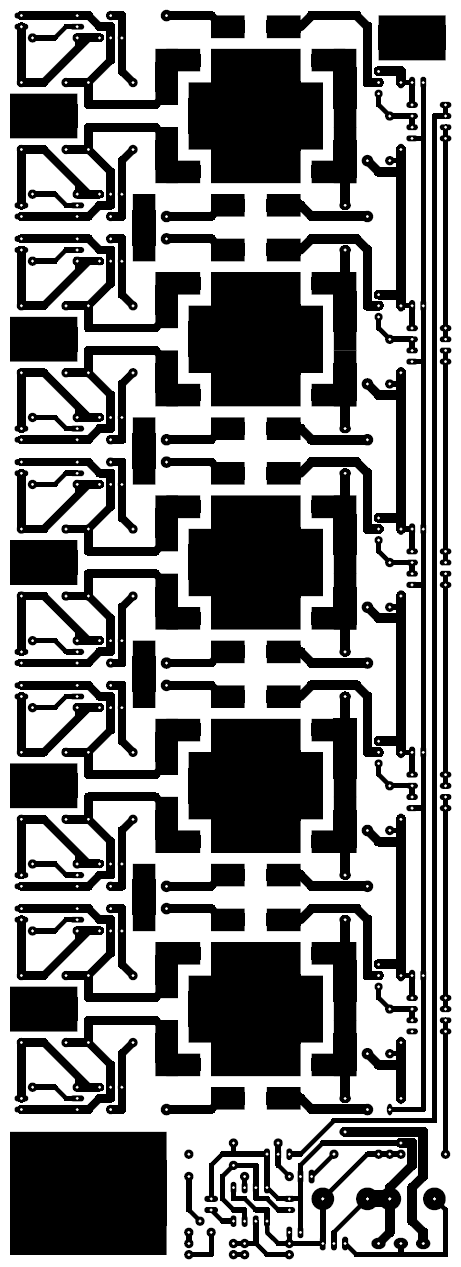
\includegraphics[width=8cm,height=18cm]{figures/design.png}
		\end{center}
			\caption{Driver Supply PCB Design}
	\end{figure}
\end{minipage}

\clearpage

\section{Hardware Realization}
\begin{figure}[H]
	\begin{center}
		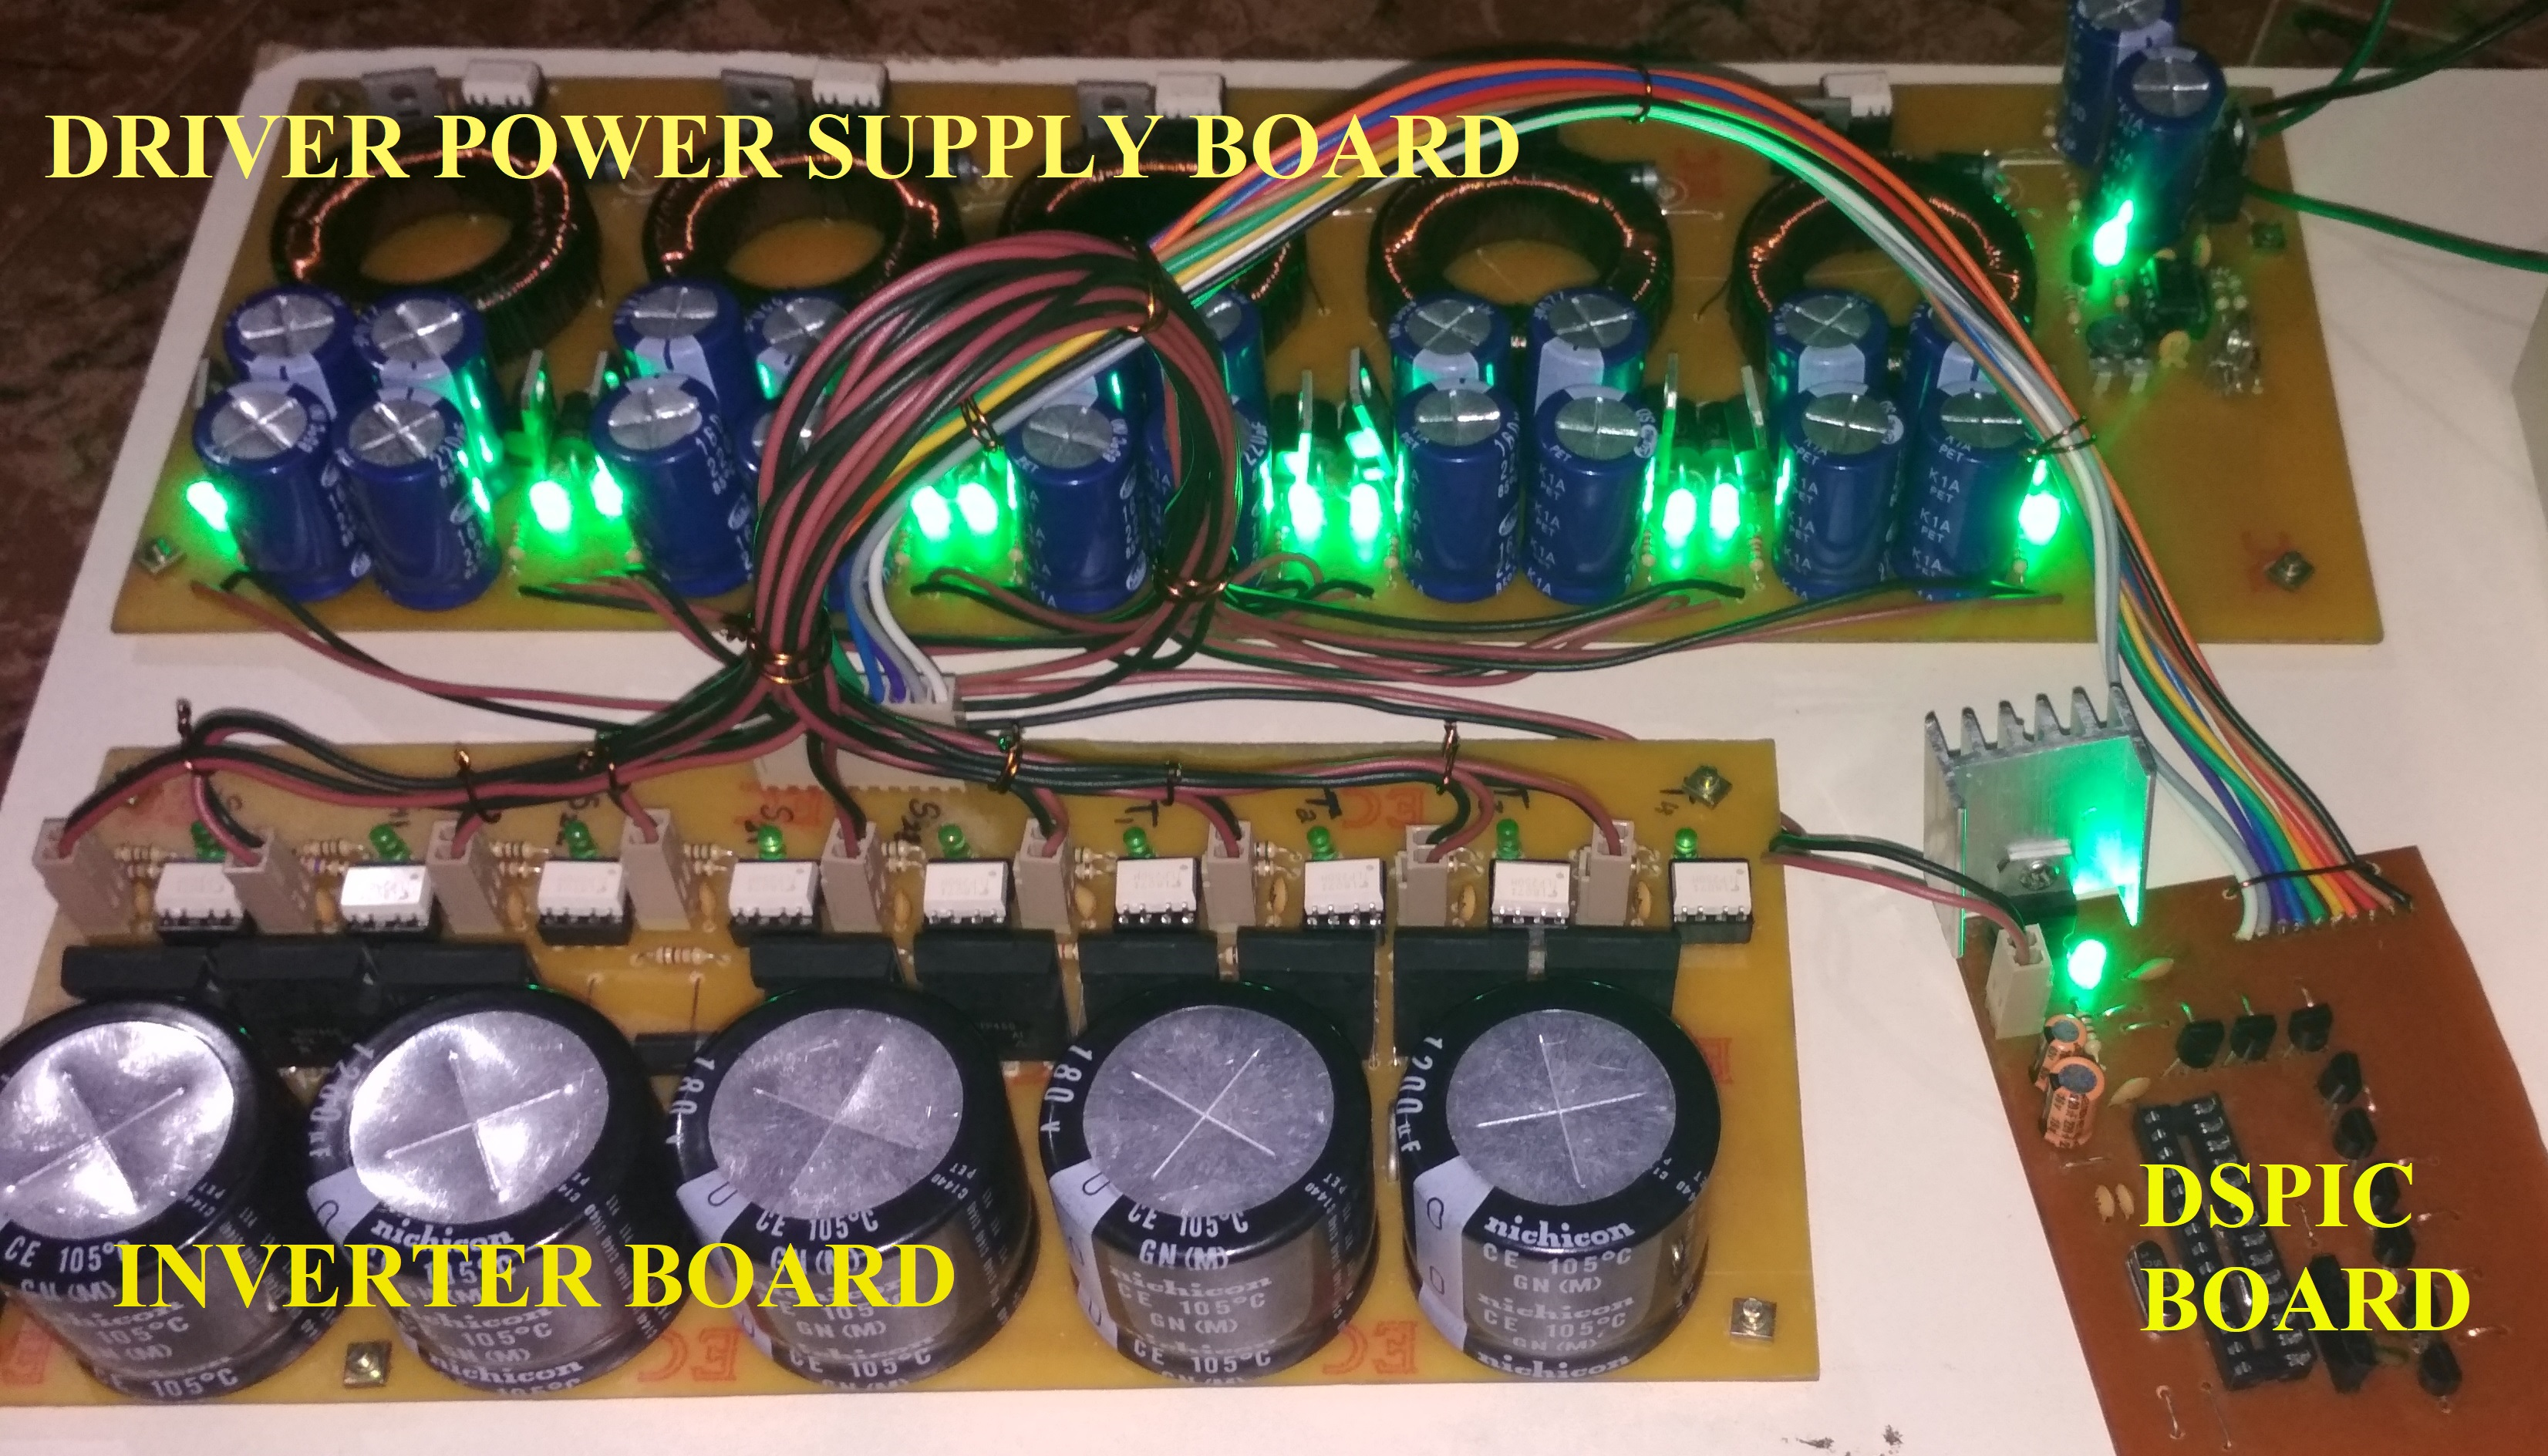
\includegraphics[width=16cm,height=9cm]{figures/HARD.jpg}
	\end{center}
	\caption{Nine level inverter hardware}
\end{figure}

The hardware realisation consists of the integration of 3 circuits, namely:\\
1. Driver power supply board.\\
2. Inverter board.\\
3. DSPIC Board.\\

The driver power supply board takes the 24 V supply from the source and then converts it into 20V and is then further regulated to obtain 15V output. The 15V output of the driver power supply board acts as the source of power for the 9 TLP250 optocoupler circuits and a DSPIC. 9 separate sources are required because using a common source for multiple switches may produce internal short circuit through the source and the connected switches. The inverter board takes 36 Voltage input and converts it into 9 level PWM signal. The TLP250 are used since the IRFP460 requires high power to switch ON which cannot be provided by the output of the DSPIC.\\

\begin{figure}[H]
	\begin{center}
		\includegraphics[width=16cm,height=9cm]{figures/HAS.JPG}
	\end{center}
	\caption{Hardware}
\end{figure}

The DSPIC30F2020 is programmed to excite the switches in the inverter depending upon the way in which it is programmed. The DSPIC30F2020 produces voltage in the output pins in the range of 5V which is given to TLP250 where the 5V pulse is converted into 15V pulses by the 15V input given to the TLP250 from the driver power circuits.\\

\clearpage

\section{Results}
\begin{figure}[H]
	\begin{center}
		\includegraphics[width=16cm,height=18.5cm]{figures/out.png}
	\end{center}
	\caption{Output voltage waveform for R load (R=100$\Omega$)}
\end{figure}
\begin{figure}[H]
	\begin{center}
		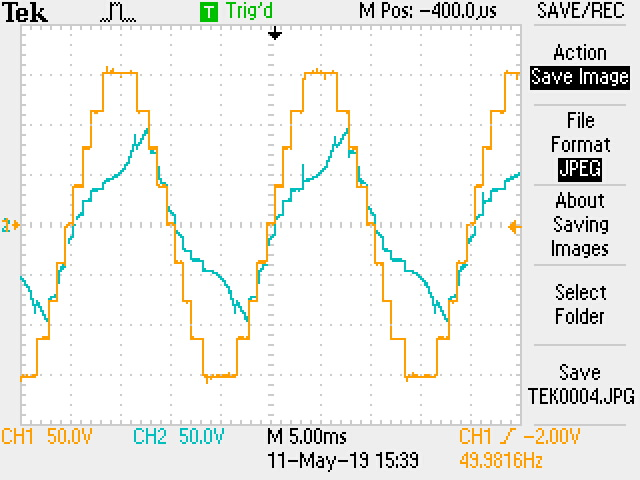
\includegraphics[width=16cm,height=9cm]{figures/HPF.JPG}
	\end{center}
	\caption{Output voltage and current waveforms for RL load (R=300$\Omega$, L=20mH)}	
\end{figure}
\begin{figure}[H]
	\begin{center}
		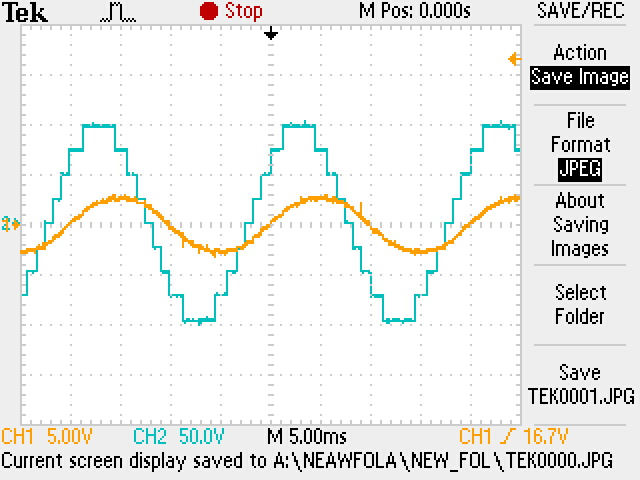
\includegraphics[width=16cm,height=9cm]{figures/LPF.JPG}
	\end{center}
		\caption{Output voltage and current waveforms for RL load (R=100$\Omega$, L=40mH)}
	\end{figure}

The peak to peak value of the inverter output wave was found to be 300 volts. When no PWM was done, the output current could only be filtered by very low power factor loads. But when PWM was given the current distortion was easily reduced at high power factor loads itself. This is due to the high frequency switching which shifts the harmonics into higher order which can easily be filtered out by very low inductance. Therefore almost the entire voltage could be applied across the R load rather than dropping a main portion of it in the inductance.
Moreover the nine level switching levels further reduce the harmonic content in the output voltage due to which satisfactoy filtering is obtained at low switching frequencies like $5khz$. The RMS voltage of $100V$ and power rating of $100W$ was found to be in agreement with the simulation model.

\chapter{CONCLUSION}
\hspace{0.1in} In this project, simulation and hardware implementation of a single-phase nine-level inverter based on switched capacitor structure has been done. This converter has a single DC source and less number of power semiconductor switches compared to nine-level diode clamped/flying capacitor/cascaded H-bridge configurations. Hence the size and cost of the converter is reduced. The peak load voltage is $4V_{in}$. Efficiency of the converter is found to be 95\%. While using PDPWM method for generation of switching signals with a switching frequency of 5kHz, the total harmonic distortion in load voltage and current are obtained 13.92\% and 1.013\% respectively. The voltage stress across the switches $S_{11}$, $S_{12}$ are $V_{in}$, $S_{21}$, $S_{22}$, $S_{23}$ are $2V_{in}$ and $T_1$, $T_2$, $T_3$, $T_4$ are $4V_{in}$. The THD in the load current can be further reduced by providing a first order filter. The main disadvantage of this converter is that the voltage stress of the H-bridge switches is equal to the peak output voltage. This converter is very suitable for low power applications with single phase system. By extending the number of levels to 17, the output current can be made nearly sinusoidal. 

\addcontentsline{toc}{chapter}{References}
\bibliographystyle{ieeetr}
\bibliography{Report}
\nocite{ngo2018single}
\nocite{williams2006principles}
\nocite{ye2014step}
\nocite{bhagyalakshmi2017switched}
\nocite{rodriguez2002multilevel}
\nocite{kouro2010recent}
\nocite{hinago2011switched}
\end{document}

